\documentclass{article}
\usepackage{amsmath, amsthm, amssymb, amsfonts, mathtools,enumitem, stmaryrd,physics, cancel, tikz-cd, graphicx, float, booktabs}
\usetikzlibrary{arrows}
\usepackage{geometry}
    \geometry{
        a4paper,
        left = 40mm,
        top = 20mm,
        right = 40mm,
        bottom = 30mm
    }
\setlength{\parindent}{0pt}

\theoremstyle{definition}
\newtheorem{problem}{Problem}
\newtheorem{solution}{Solution}
\newtheorem*{example}{Example}
\newtheorem*{exercise}{Exercise}
\newtheorem*{definition}{Definition}
\newtheorem{theorem}{Theorem}
\newtheorem*{theorem*}{Theorem}
\newtheorem{proposition}[theorem]{Proposition}
\newtheorem*{proposition*}{Proposition}
\newtheorem{lemma}[theorem]{Lemma}
\newtheorem*{lemma*}{Lemma}
\newtheorem{corollary}[theorem]{Corollary}
\newtheorem*{corollary*}{Corollary}
\newtheorem*{remark}{Remark}

\title{M623 Geometric Topology I}
\author{Thanic Nur Samin}
\date{}


\begin{document}
    \maketitle

    \section*{Monday, 8/25/2025}

    Textbook: \textit{Characteristic Classes} by Milnor and Stasheff. Hereafter referred by MS.

    \underline{Read Chapter 1 and 2 of MS.}

    \begin{definition}
        [\(n\)-manifold]

        Two different variants: embedded and abstract.

    

        Abstract: \((M, \mathcal{A})\) where \(\mathcal{A}\) is an atlas.
    \end{definition}

    Embedded: \(M \subset \mathbb{R}^A\). Here, \(A =\) index set, \(\mathbb{R}^A = \text{func}(A,\mathbb{R})\) with the product topology.

    \(M\) Hausdorff space, \(U \subset M\) open, \(V \subset \mathbb{R}^n\) open.
        
    Chart \(\phi : U \xrightarrow{\approx} V\) homeomorphism.

    Parameterization (ptz) \(h: V \xrightarrow{\approx} U\)

    We want some calculus.

    Let open \(V \subset \mathbb{R}^n\).

    A function \(f: V \to \mathbb{R}\) is \textit{smooth} if all partials of all orders exist: \(\frac{\partial^k f}{\partial x_{i_1} \cdots \partial x_{i_{p}}}\).

    \(f: V \to \mathbb{R}^A\) is \textit{smooth} if \(f_\alpha\) smooth \(\forall \alpha \in A\).

    \[
        \begin{tikzcd}
            V \ar[rr, bend right,"f_\alpha"'] \ar[r,"f"] & \mathbb{R}^A \ar[r,"pr_{\alpha}"] & \mathbb{R}
        \end{tikzcd}
    \]

    We can go from abstract manifold to embedded manifold.

    Let \(A = C^{\infty} (M,R)\).

    \(M \xrightarrow{i}\mathbb{R}^A\) where \(i(x) = (f \mapsto f(x))\).

    We can go to the reverse direction easily once we have all the definitions.

    \begin{definition}
        Two charts \((\phi_1: U_1 \to V_1)\) and \((\phi_2: U_2 \to V_2)\) are compatible (or smoothly compatible) if \(\phi_2 \circ \phi_1 ^{-1}\) is smooth. Explicitly,

        \(\phi_1(U_1 \cap U_2) \xrightarrow{\phi_2 \circ \phi_1 ^{-1}} \phi_2(U_1 \cap U_2)\) needs to be smooth. 
    \end{definition}

    \begin{definition}
        Parameterization \(h: V \to U\) is \textit{smooth} (assume \(M \subset \mathbb{R}^A\)) if:

        \[
            \begin{tikzcd}
                V \ar[r,"h"] \ar[rrr, bend right,"h"] & U \ar[r,hook] & M \ar[r,hook] & \mathbb{R}^n
            \end{tikzcd}
        \]

        is smooth.

        and has rank \(n\). ie, \(\forall v\in V\) the Jacobian:

        \[
            dh = \left( \frac{\partial_\alpha h}{\partial x_j}(v) \right)
        \]
    
        has rank \(n\).

        eg \(x \mapsto x^3\) is a parameterization which is not smooth, since the Jacobian has rank \(0\) at \(0\).
    \end{definition}

    Now we can properly define manifolds.

    \begin{definition}
        [Embedded Smooth \(n\)-Manifold] \(M \subset \mathbb{R}^A\) so that \(\forall x\in M\) there exists a smooth rank \(n\) parameterization \(h : V \to U \ni x\).

        We assume \(M\) is Hausdorff.
    \end{definition}

    We can now define a Cateogry of Embedded Manifolds.

    \begin{definition}
        [Category of Embedded Manifolds] \(\operatorname{Embmfld}\).

        \underline{Objects}: embedded \(M \subset \mathbb{R}^A\) of \(\dim n\) for some \(n\).

        \underline{Morphisms}: Smooth Maps (has to be defined carefully, restricting in Euclidean space).

        Diffeomorphism = invertible morphism.
    \end{definition}

    Let \((M \subset \mathbb{R}^A), (N \subset \mathbb{R}^B)\). \(f: M \to N\) is smooth if \textit{locally smooth}, meaning \(\forall x\in M, \exists\) smooth parameterization \(h: V \to U \ni x\) such that \(V \to U \hookrightarrow M \xrightarrow{f} N \to \mathbb{R}^B\) is smooth.

    Now we can define abstract manifold independend of embedded manifolds.

    \begin{definition}
        [Abstract Manifold] Let \(M\) be Hausdorff. An \(n\)-\textit{atlas} on \(M\) is a set \(\mathcal{A}=\left\{ \phi_\alpha : U_\alpha \xrightarrow{\approx} V_\alpha \subset \mathbb{R}^n \right\}\) of compactible \(n\)-charts such that \(\{ U_\alpha \} \) covers \(M.\)

        Atlas \(\mathcal{A}\) and \(\mathcal{A}^{\prime}\) are \underline{compatible} if all charts are.

        Fact: Every atlas is contained in a unique maximal atlas.

        Then an abstract manifold is \((M,\mathcal{A})\) with a maximal \(n\)-atlas.
    \end{definition}

    \section*{Wednesday, 8/27/2025}
    
    Recall: embedded \(n\)-manifold \(M \subset \mathbb{R} ^ A\): \(\forall x\in M, \exists\) smooth, rank \(n\) parameterization \(h: V \to U \subset M\) such that \(x\in U\). We assume \(M\) is Hausdorff.

    Abstract \(n\)-manifold: \((M, \mathcal{A})\) where \(\mathcal{A}\) is an \(n\)-atlas, so \(\mathcal{A}  = \{ \text{charts } \phi_\alpha : U_\alpha \xrightarrow{\cong} V_\alpha \}\) such that \(\{ U_\alpha \}\) cover \(M\) and \(\{ \phi_\alpha \} \) smoothly compatible. We assume \(M\) is Hausdorff.
    
    \begin{remark}
        If we have an abstract manifold we have a surjective map \(\coprod V_\alpha \overset{\coprod \phi_\alpha ^{-1}}{\twoheadrightarrow} M\).
        
        Then we can define \(M \cong \frac{\coprod V_\alpha}{\sim}\). This gives us another definition of a manifold. 
    \end{remark}

    \begin{exercise}
        Define smooth \(f: (M,\mathcal{A}) \to (N,\mathcal{B})\).

        Not hard, just annoying to get the definitions right!
    \end{exercise}

    \begin{theorem}
        Categories of abstract manifolds and embedded manifolds are equivalent.

        \[
            \text{EmbMflds} \simeq \text{absMflds}  
        \]
    \end{theorem}

    Recall equivalent categories:

    \begin{definition}
        Categories \(\mathcal{C}\) and \(\mathcal{D}\) are equivalent (Notation: \(\mathcal{C} \simeq \mathcal{D}\)): If there are functors \(\mathcal{C} \xrightarrow{F} \mathcal{D}\) and \(\mathcal{D} \xrightarrow{G} \mathcal{C}\) such that \(F \circ G\) and \(G \circ F\) are naturally isomorphic to the respective identities.
    \end{definition}

    We need some more definitons.

    \begin{definition}
        A skeleton of \(\mathcal{C}\) is \(\operatorname{Sk} \mathcal{C} \subset \mathcal{C}\) is a full subcategory \(\forall c\in \mathcal{C}, \exists ! c^{\prime} \in \operatorname{Sk} \mathcal{C}\) such that \(c \cong c^{\prime}\).

        \(\mathcal{A} \subset \mathcal{B}\) is full if \(\forall a,a^{\prime} \in \operatorname{Ob} \mathcal{A}, \mathcal{A}(a,a^{\prime}) \xrightarrow{\cong} \mathcal{B}(a,a^{\prime})\) 
    \end{definition}

    For example, let \(\mathcal{C} =\) finite sets. Then \(\operatorname{Sk} \mathcal{C} = \{ 1 \}, \{ 1,2 \}, \{ 1,2,3 \}, \cdots\) 

    \begin{theorem}
        \(\mathcal{C} \simeq \mathcal{D} \iff \operatorname{Sk} \mathcal{C} \cong \operatorname{Sk} \mathcal{D}\).
    \end{theorem}

    Note that \(\mathcal{C} \simeq \operatorname{Sk} \mathcal{C}\) so one direction is trivial.

    \begin{lemma}
        [1.1] Let \(h\) and \(h^{\prime}\) be smooth rank \(n\) on \(M \subset \mathbb{R}^A\). Then \(h ^{-1} \circ  h^{\prime}\) is smooth (thus a diffeomorphism).
        
        Let \(V\) and \(V^{\prime}\) be the domain of \(h\) and \(h^{\prime}\) respectively. Then \(h ^{-1} \circ h^{\prime} : (h^{\prime})^{-1} (V\cap V^{\prime}) \to h ^{-1} (V \cap V^{\prime})\) 
    \end{lemma}

    \begin{corollary}
        \(\mathcal{A} = \{ h ^{-1} \mid h \text{ parameterization} \}\) is \(n\)-atlas on \(M\).

        This gives us \(\text{EmbMflds}\to \text{AbstMflds}\).
    \end{corollary}

    \begin{proof}
        This is the proof of lemma 1.1, lemma 3 in the notes.

        Assume \(V = V^{\prime}\). WTS: \((h^{\prime})^{-1} V \to h ^{-1} (V)\) is smooth.

        For \(x\in V\) choose \(\alpha_1, \cdots , \alpha_n \in A\) such that \(\det \left( \frac{\partial \alpha_i}{\partial x_j} (x) \right)  \not\equiv 0\). 

        We have:

        \[
            \begin{tikzcd}
                M \ar[r, hook] & \mathbb{R}^A \ar[d, "pr_{\alpha_1 \cdots \alpha_n}"] \\ V \ar[u,"h"] \ar[r,dotted] & \text{subset of } \mathbb{R}^n
            \end{tikzcd}
        \]

        Then, by the inverse function theorem, the dotted map is locally invertible.

        \(h^{-1} \circ h^{\prime} = (pr \circ inc \circ h)^{-1} \circ inc \circ pr \circ h^{\prime}\) near \(h ^{-1} x\).

    \end{proof}

    Given abstract \((M,\mathcal{A})\), let \(A = C^{\infty} (M,\mathbb{R})\) smooth functions.
    
    \(i: M \to \mathbb{R}^A, x \mapsto (f \to f(x))\).
    
    Let \(M_1 = i(M)\).
    
    \begin{lemma}
        [1.5] \(M_1 \subset \mathbb{R}^A\) is \(\text{EmbMfld}\). \(M \xrightarrow{i} M_1\) is diffeomorphism.
    \end{lemma}

    \subsection*{Definition of tangent vector, tangent space and tangent bundle}

    \begin{definition}
        [Tangent Vector] is velocity vector of a curve.

        We have defined morphisms. Consider the embedded case: suppose we have smooth \(\gamma : \mathbb{R} \to M \subset \mathbb{R}^A\). Then,

        \[
            \gamma^{\prime} (0) = \lim_{h \to 0} \frac{\gamma (h) - \gamma(0)}{h} \in \mathbb{R}^A
        \]

        is a tangent vector
    \end{definition}

    \begin{definition}
        [Tangent Space] Suppose \(x\in M \subset \mathbb{R}^A\), an \(n\)-dim embedded manifold. \(T_x M =\) tangent space of \(M\) at \(x\). This is:
        
        \[
            \left\{ \gamma ^{\prime} (0) \mid \gamma(0) = x \right\} \subset \mathbb{R}^A
        \]

        an \(n\)-dim subspace.
    \end{definition}

    We are going to bundle this together.

    \begin{definition}
        [Tangent Bundle]

        \(TM = \left\{ (x,v) \in M \times \mathbb{R}^A \mid v\in T_x M \right\}\).

        By definition, \(TM \subset M \times \mathbb{R}^A\) so this is in fact a topological space.

        We have a projection map \(TM \xrightarrow{\pi} M\) by \((x,v) \mapsto x\).
    \end{definition}

    \begin{remark}
        Fibers of \(\pi\), \(\pi ^{-1} (x)\) are vector spaces: \(\pi ^{-1} (x) = T_x M\).

        Then, \(TM = \bigcup_{x\in M} \{ x \} \times T_x M\).

        Abuse of notation lets us write this as \(\bigcup T_x M\).

        Thus, tangent bundle is in fact a bundle of tangents.
    \end{remark}

    What about abstract manifolds \((M,\mathcal{A})\)?

    We can define \(TM\) as follows:

    \begin{itemize}
        \item \(M \subset \mathbb{R}^{C^{\infty}(M,\mathbb{R})}\).
        \item \(TM = \frac{\coprod V_\alpha \times \mathbb{R}^n}{\sim}\)
        \item \(T_x M =\) velocity vector of curves.
        \item derivations.
    \end{itemize} 

    Suppose we have smooth function between manifolds \(f: M \to N\). \(\forall x\in M\) we can define linear \(\mathrm{d}f_x : T_x M \to T_{f(x)} N\), \(\gamma ^{\prime} (0) \mapsto (f \circ \gamma)^{\prime} (0)\). \(\mathrm{d} f_x\) is a map between vector spaces, so it is a linear transformation. It is the `Jacobian'.
    
    Then we have \(\mathrm{d} f: TM \to TN\) such that \(\mathrm{d} f(x,v) = \mathrm{d} f_x(v)\).

    We also have the chain rule: \(\mathrm{d} (f \circ g) = \mathrm{d} f \circ \mathrm{d} g\) 

    \section*{Friday, 8/29/2025}
    
    No class next week!

    Manifold constructed by:

    \begin{itemize}
        \item open subset of \(\mathbb{R}^n\)
        \item Subset double torus \(\subset \mathbb{R}^3\)
        \item Quotients: \(P^n = \mathbb{R} P^n = S^n / x \sim -x\)
        \item Lie groups/ matrix group, eg closed subgroups of \(\operatorname{GL}_n\mathbb{R} \underset{\text{open}}{\subset} M_n \mathbb{R} = \mathbb{R}^{n^2}\) 
        \item Zero sets.
        \begin{itemize}
            \item regular values
            \item transversality
            \item smooth varieties 
        \end{itemize} 
    \end{itemize} 

    \begin{definition}
        \(t_0\in \mathbb{R}\) is a regular value of \(f: M \to \mathbb{R}\) if \(\forall x\in f ^{-1} t_0, \mathrm{d}f_x\) is onto.
    \end{definition}

    \(f^{-1}(\text{regular value})\) is a submanifold of \(M\).

    Consider \(S^n \subset \mathbb{R}^{n+1}\), and \(f: \mathbb{R}^{n+1} \to \mathbb{R}\) given by \(x \mapsto x_1^2 + \cdots + x_{n+1}^2\).

    \(1\) is a regular value \(f ^{-1} 1 = S^n\).

    \begin{definition}
        Let \(f: M \to N \supset X\) submanifold.

        \(f\pitchfork X\), \(f\) is \textit{transverse} to \(X\) if \(\forall m \in f ^{-1} X, T_{f(m)}N = T_{f(m)} X + \mathrm{d}f_m (T_m M)\).
    \end{definition}

    \begin{figure}[H]
        \centering
        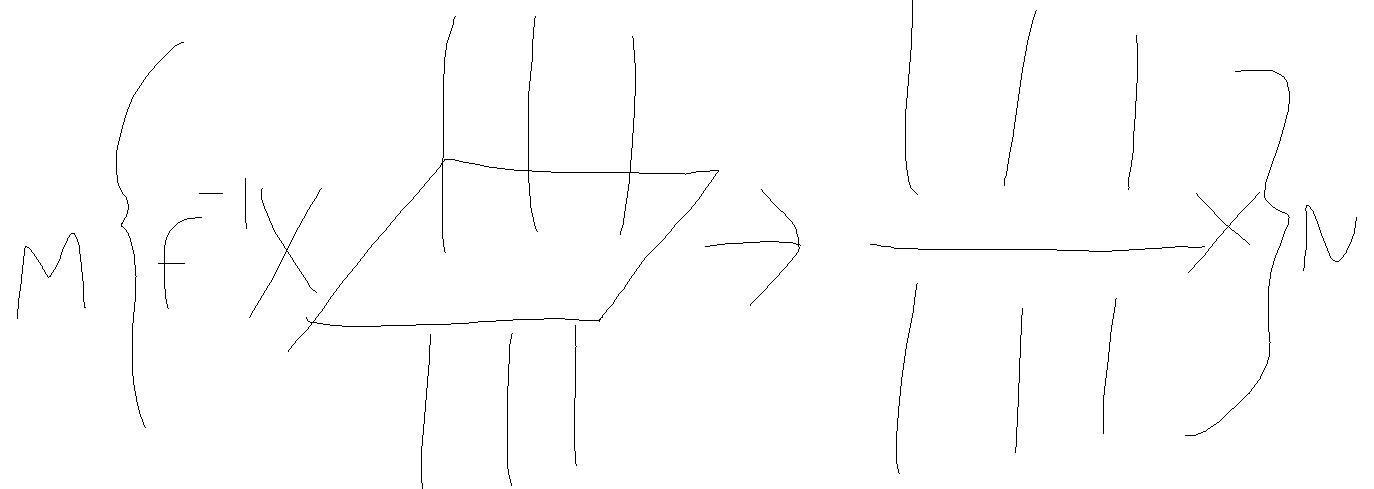
\includegraphics[width=0.8\textwidth]{img/transverse}
        \caption{}
        \label{fig:}
    \end{figure}

    \begin{theorem}
        \(f ^{-1} X\) is a submmanifold of \(M\).

        Furthermore, \(\dim N - \dim X = \dim M - \dim f ^{-1} X\).
    \end{theorem}

    In fact, \(\nu (f ^{-1} X \hookrightarrow M) \to \nu (X \hookrightarrow N)\) as vector space isomorphism on fibers.

    [insert picture later]

    Now, suppose \(F\) is a topological space.

    \begin{definition}
        A fiber bundle with fiber \(F\):

        Let \(E \xrightarrow{\pi} B\) be a continuous map suuch that \(\forall b\in B, \exists\) open \(b\in U \subset B\) and:

        \[
            \begin{tikzcd}
                U \times F \ar[rr, "h", "\approx"'] \ar[rd, "pr_U"] && \pi ^{-1} U \ar[ld,"\pi"] \\ & U 
            \end{tikzcd}
        \]

        \(h\) fiber preserving homeomorphism. \(\forall b^{\prime} \in U\), \(F \cong F \times b^{\prime} \xrightarrow{\approx} F_{b^{\prime}} \coloneqq \pi ^{-1} (b^{\prime})\).
    \end{definition}

    Write: \( \begin{tikzcd}
        F \ar[r] & E \ar[d] \\ & B 
        \end{tikzcd} \)

    \[
        \begin{tikzcd}
            I \ar[r] & Mob \ar[d] \\ & S^1
        \end{tikzcd}
    \]

    eg \(B \times F \to B\) trivial bundle.

    \section*{Chapter 2 of MS}

    \begin{definition}
        A real vector bundle \(\xi\) over \(B\) is:

        \[
            \xi = \left( \begin{tikzcd} E \ar[d,"\pi"] \\ B \end{tikzcd}, \forall b\in B, \pi ^{-1} b = F_b \text{ is a fin. dim vector space.} \right) 
        \]

        \(F_b \times F_b \to F, \mathbb{R} \times F_b \to F\) satisfies \(8\) axioms s.t.

        \(\forall b\in B, \exists b\in U \subset B\) and \(n\geq 0\) and \(\begin{tikzcd}U \times \mathbb{R}^n \ar[rr,"h","\approx"'] \ar[rd] && \pi ^{-1} U \ar[ld] \\ & U\end{tikzcd}\).
    
        \(\mathbb{R}^n \cong b \times \mathbb{R}^n \xrightarrow[\approx]{h} \pi ^{-1} b\) is an isomorphism of vector spaces.
    \end{definition}

    If \(B\) is connected then \(n\) is constant.

    `rank \(n\) vector bundle'.

    \(n\)-plane bundle.

    Another thing MS does is write this: \(\xi = \begin{tikzcd} E(\xi) \ar[d,"\pi(\xi)"] \\ B(\xi)\end{tikzcd}\) for vector bundle which is very precise.

    \subsection*{Isomorphism of vector bundles over \(B\)}.

    Consider two bundles \(\xi\) and \(\eta\) and we have the homeomorphism

    \[
        \begin{tikzcd}
            E(\xi) \ar[rr, "\approx"] \ar[rd] && E(\eta) \ar[ld] \\ & B
        \end{tikzcd}
    \]

    vector space isomorphism on the fibers.

    \subsection*{Examples of vector bundles}

    We have the trivial bundle \(\begin{tikzcd} B \times \mathbb{R}^n \ar[d,"\underline{\mathbb{R}^n} = \underline{\mathbb{R}}^n_B = \varepsilon^n_B ="'] \\ B \end{tikzcd}\) 

    We have tangent bundles:

    \[
        \tau_M = \left\{ \begin{tikzcd} TM \ar[d,"\pi"] \\ M \end{tikzcd} , T_x M \right\} 
    \]

    \begin{definition}
        \(M\) is parallelizable if \(\tau_M\) is trivial.
    \end{definition}

    \(S^1\) is paralellizable.

    Lie groups are parallelizable eg \(S^3\).

    \(S^2\), or \(S^{2n}\) in general not parallelizable via the hairy ball theorem.

    We also have normal bundles. Consider \(M \subset \mathbb{R}^N\).

    \(\nu(M \subset \mathbb{R}^n) = \{ (x,v) \in M \times \mathbb{R}^n \mid x \in M, v \in (T_x M)^{\perp}\}\)
    
    \(\nu (S^2 \hookrightarrow S^3) \leftarrow S^2 \times \mathbb{R}\) is trivial, the map is \((x,tx) \mapsfrom (x,t)\).

    Tautological bundle over \(P^n\): \(\gamma_n^1 = \begin{tikzcd}
        \mathbb{R} \ar[r] & E(\gamma_n^1) \ar[d] \\ & P^n
    \end{tikzcd}\) 

    Note that \(P^n = S^n / x \sim -x =\) lines through \(O\) in \(\mathbb{R}^{n+1}\).

    \(E(\gamma_n^1) = \left\{ (\{ x,-x \}, v) \in P^n \times \mathbb{R}^{n+1} \mid v \in \mathbb{R} x \right\}\).

    \(E(\gamma_n^1) \xrightarrow{\pi} P^n, (\{ x,-x \} \mapsto \{ x,-x \})\). Essentially, point on line \(\mapsto\) line. 

    This tautological bundle is non-trivial.

    \section*{Monday, 9/8/2025}
    
    Last week was a break.

    HWK: an exercise from ch2. (C, D, E are recommended).

    Recall: a vector bundle \(\xi\) is \begin{tikzcd} \mathbb{R} \ar[r] & E \ar[d,"\pi"] \\ & B\end{tikzcd} meaning fibers of \(\pi\) are \(k\)-dimensional vector spaces.

    \begin{definition}
        A section of \(\xi\) is actually a section of \(\pi\).

        \(s: B \to E\) such that \(\pi \circ s = \operatorname{id}_{B}\).
    \end{definition}

    Section looks like this:

    \[
        \begin{tikzcd}
            \mathbb{R}^k \ar[r] & E \ar[d,"\pi"] \\ & B \ar[u, dotted, bend left, "s"]
        \end{tikzcd}
    \]

    Section of \(TM \eqqcolon\) vector field.

    There's also the zero section \(z: B \to E\) given by \(b \mapsto 0 \in \pi ^{-1} b\).

    \(\begin{tikzcd} E \ar[d,"\pi"] \\ B \ar[u,bend left, dotted,"z"] \end{tikzcd}\) homotopy inverses.

    Now we show there is some twisting.

    \(\begin{tikzcd} E_0 \ar[d] & = E - z(B) \\ B \end{tikzcd}\). \(B\) trivial implies \(E_0 \cong B \times (\mathbb{R}^k \setminus  e) \simeq B \times S^{k-1}\).

    We have the tautological line bundle:

    \[
        \begin{tikzcd}
            R \ar[r] & E \ar[d] & = \{ ([x],v) \mid v\in \mathbb{R} x \} & \subset P^n \times \mathbb{R}^{n+1} \\ & P^n & = S^n / x \sim -x 
        \end{tikzcd}
    \]

    We can think of it like \((\text{line}, \text{point on line}) \in E\).
    
    For example, consider \(P^1\). This gives us the open mobius strip.

    \begin{theorem}
        [2.1] \(\gamma_n^1\) is nontrivial for \(n \geq 1\).
    \end{theorem}

    \begin{proof}
        \(E(\gamma_n^1)_0\) is connected \(\iff \not\simeq P^n \times S^0\).
    \end{proof}

    \begin{figure}[H]
        \centering
        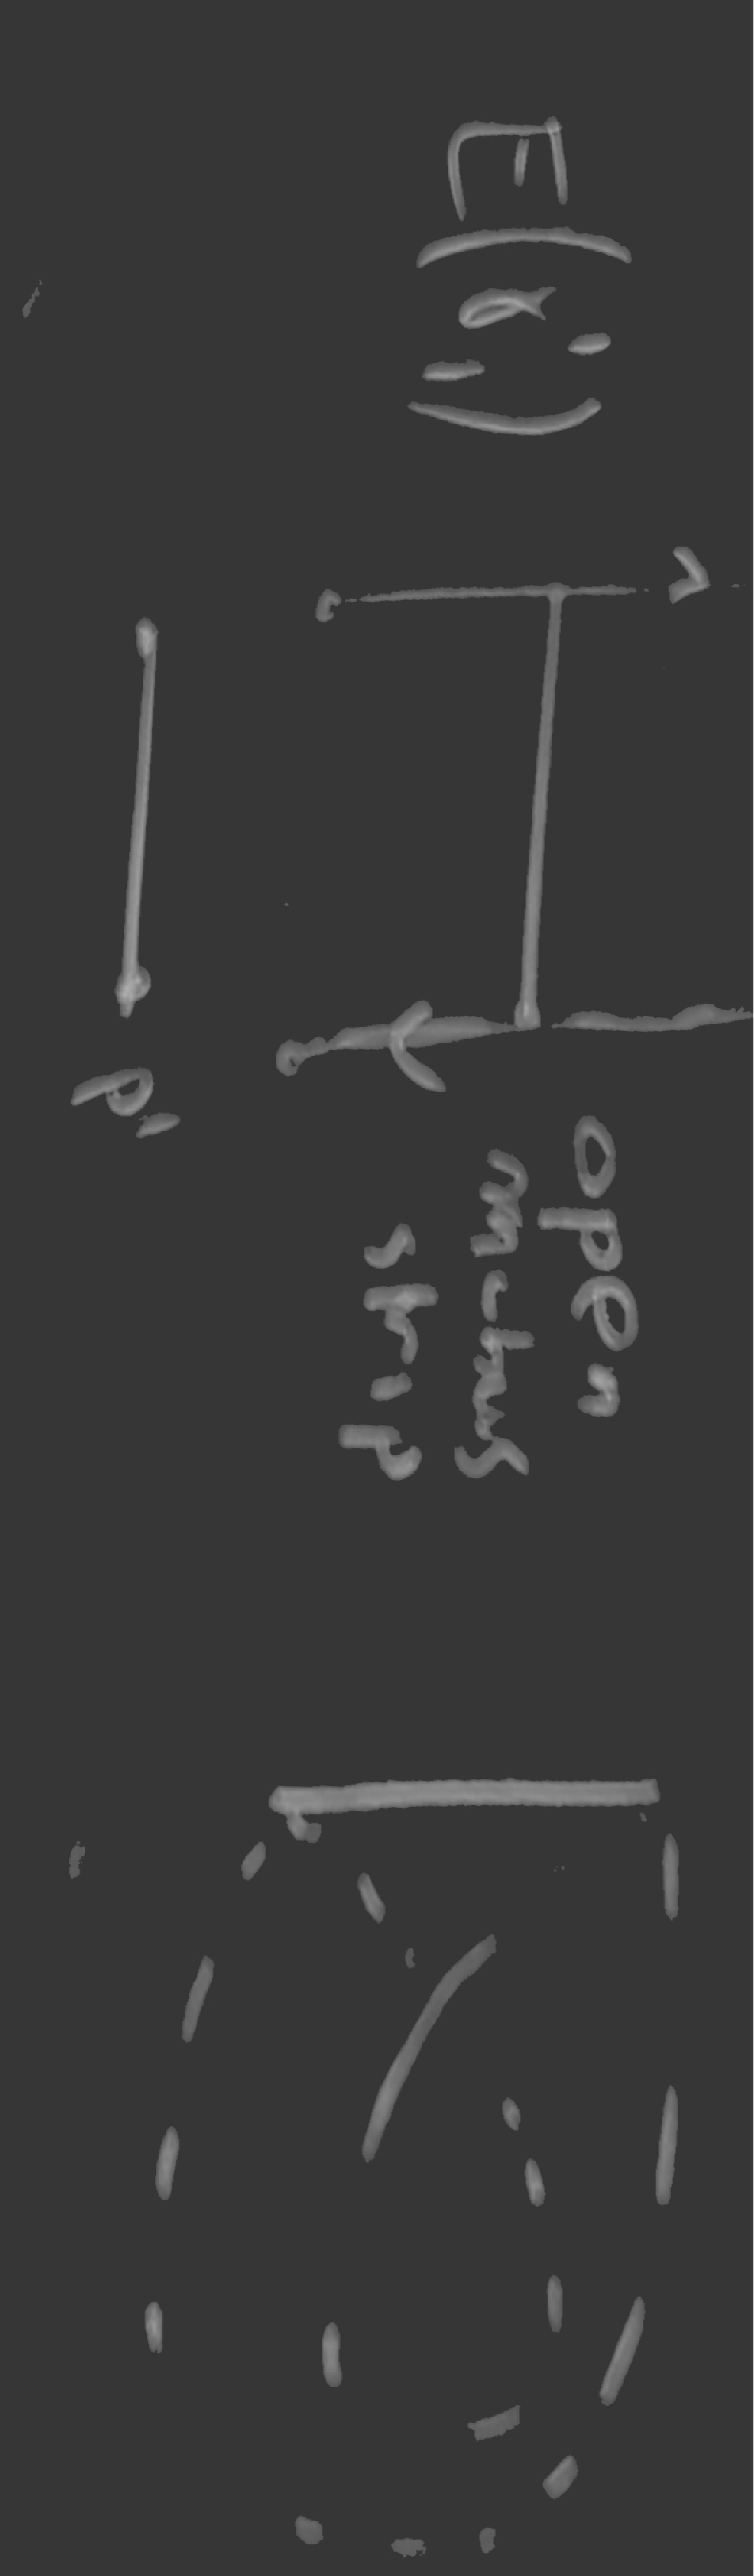
\includegraphics[height=0.8\textwidth, angle=90]{img/gamma11.pdf}
        \caption{}
    \end{figure}

    \begin{definition}
        A metric on a vector bundle \(\xi \) is \(g: E \times_B E \to \mathbb{R}\) such that \(\forall b\in B, \pi ^{-1} b \times \pi ^{-1} b \to \mathbb{R}\) is an inner product.
    \end{definition}

    Recall: pullback of \(\begin{tikzcd}
        & B\ar[d,"\beta"] \\ A \ar[r,"\alpha"] & C
    \end{tikzcd}\) is \(A \times_C B = \left\{ (a,b) \mid \alpha (a) = \beta(b) \right\} \subset A \times B\).

    Also see: a vector bundle \(E \to B\) needs all fibers to be vector spaces. For a metric we want them to be inner product spaces.

    A bundle with metric is often callled a Euclidean vector bundle.

    Examples: A \textit{Riemannian manifold} is \(TM\) with a smooth metric [\(g\) is smooth].

    If \(M^n \subset \mathbb{R}^N\) we can use the inner product inherited from \(\mathbb{R}^N\) so it is a riemannian manifold.

    eg the trivial bundle has a metric: \((B \times \mathbb{R}^n) \times_B (B \times \mathbb{R}^n) \to \mathbb{R}^n\) which looks like \(((b,v),(b,w)) \mapsto v \cdot w\). 

    If \(M^n \subset \mathbb{R}^N\), \(TM = \left\{ (x,v) \in M \times \mathbb{R}^N \mid v = \gamma^{\prime} (0), \gamma(0) = x \right\} \) 

    \(\lVert (x,v) \rVert = \lVert v \rVert, g((x,v),(x,w)) = v \cdot w\).

    Then \(\lVert \cdot \rVert : E \to \mathbb{R}_{\geq 0}\) given by \(\lVert v \rVert \coloneqq \sqrt{g(v,v)}\).

    \begin{theorem}
        [Exercises, ch2] Suppose \(B\) is paracompact. We can look at Isomorphism classes of Euclidean vector bundles over \(B\), forget the metric to get isomorphism classes of vector bundles over \(B\):

        \[
            \begin{Bmatrix}
                \text{iso class of euclidean} \\
                \text{vector bundle over \(B\)} 
            \end{Bmatrix} \xrightarrow{\text{forget } g}\begin{Bmatrix}
                \text{iso class of} \\
                \text{vector bundle over \(B\)} 
            \end{Bmatrix} 
        \]

        This is an isomorphism.
    \end{theorem}

    \begin{definition}
        Sections \(s_1, \cdots , s_n\) of rank \(n\) vector bundle \(\begin{tikzcd}
            E \ar[d] \\ B \ar[u, bend right, dotted, "s_i", swap]
        \end{tikzcd}\) are llinearly independent (l.i) if \(\forall b\in B, \left\{ s_1(b), \cdots , s_n(b) \right\} \) is linearly independent in \(\pi ^{-1} (b)\).  
    \end{definition}

    \begin{theorem}
        [2.2] rank \(n\) vector bundle \(\xi \) is trivial iff \(\xi \) has \(n\) l.i. sections.
    \end{theorem}

    \begin{proof}
        \(\implies: s_i(b) \coloneqq (b,\underline{e_i}) \in B \times \mathbb{R}^n\).
        
        \(\impliedby:\) define \(f: B \times \mathbb{R}^n \to E\) by \(\left( b, \sum a_i e_i \right) \mapsto \sum a_i s_i(b)\) 
    \end{proof}

    eg \(T^2\) has \(2\) l.i. sections, thus \(TT^2 \cong T^2 \times \mathbb{R}^2\).

    \begin{figure}[H]
        \centering
        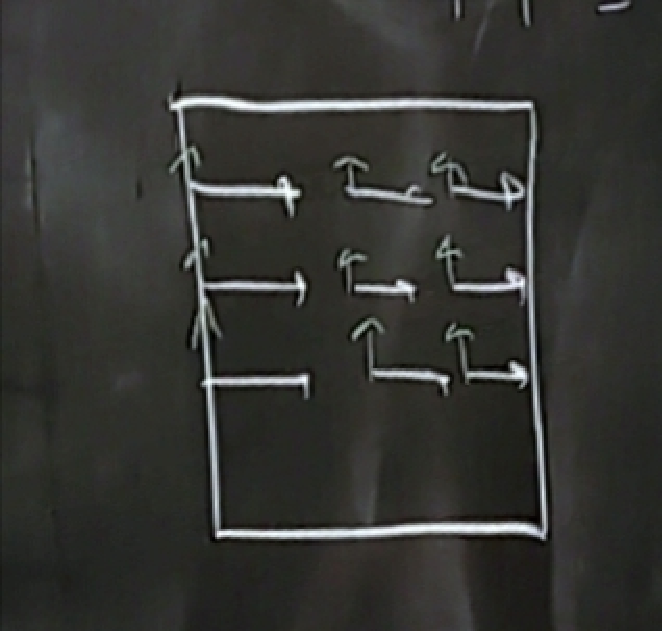
\includegraphics[width=0.3\textwidth]{img/trivialtorus}
        \caption{}
    \end{figure}

    \section*{Wednesday, 9/10/2025}
    
    \section*{Chapter 3: New bundles}

    Homeowrk: pick up problems from chapter 3 (and chapter 2).

    \textit{Abstract definition of bundle} (Steenrod, see D-Kirk 5.2).

    Let \(G\) be a topological group, \(F\) a space, \(G \curvearrowright F\)

    Topological group meaning: \(G\) topological group means \(G\) is a group and a space such that \(G \times G \to G, (a,b) \mapsto ab\) and \(G \to G, a \mapsto a ^{-1}\) are continuous.

    Action of \(G\) on \(F\): \(G \times F \to F\) given by \(ef = f\) and \((gg^{\prime})f = g (g^{\prime} f)\).

    \begin{definition}
        A fiber bundle with structure group \(G\) and fiber \(F\) [\((G,F)\)-bundle] is a map with:
        
        Map \(\begin{tikzcd}
            E \ar[d] \\ F
        \end{tikzcd}\)
        
        Atlas \(\mathcal{A} = \{ \phi : U_{\phi} \times F  \xrightarrow{\approx} \pi ^{-1} U_\phi \} \) 

        Transition functions \(\Theta = \left\{ \theta_{\phi,\psi} : U_{\phi} \cap U_{\psi} \to G \mid \phi,\psi \in \mathcal{A} \right\} \) 

        such that:

        \begin{enumerate}[label=\arabic*)]
            \item \(\{ U_{\phi} \} \) open cover of \(B\).
            \item Fiber preserving homeomorphism:
            
            the following diagram commutes: \(\begin{tikzcd}
                U_{\phi} \times F \ar[rr,"\approx"] \ar[rd] && \pi ^{-1} U_\phi\ar[ld] \\ & U_{\phi} 
            \end{tikzcd}\)   
            \item \(b \in U_{\phi}\cap U_{\psi}, f\in F \implies \psi(b,f) = \phi(b,\theta_{\phi, \psi}(b)f)\) 
            \item \(\theta_{\phi,\psi}(b) = \theta_{\phi, \chi}(b) \theta_{\chi,\psi}(b)\) 
        \end{enumerate} 
    \end{definition}

    Examples:

    \(G\) trivial group implies the bundle is a trivial bundle, \(\begin{tikzcd}
        B \times F \ar[d] \\ B
    \end{tikzcd}\) 

    \(G = \operatorname{GL}(n,\mathbb{R}), F = \mathbb{R}^n\) gives us the rank \(n\) vector bundle. Let \(b\in B\), choose \(\phi , b\in U_{\phi}\). Use the atlas to find bijection \(\pi ^{-1} b \cong \mathbb{R}^n\). This gives us a vector space on \(\pi ^{-1} b\) independent of the choice of \(U_{\phi}\) by the 3rd condition.

    If the \(G\)-action on \(F\) is \textit{effective}, meaning every non-trivial action does something, meaning there is \(f\in F\) such that \(gf\neq f\) for every \(g\in G \setminus \{ e \}\), then we don't need condition 4.

    If \(G=\operatorname{O}(n)\) and \(F=\mathbb{R}^n\) then we have a vector bundle with a metric.
    
    If \(G = \operatorname{GL}(n,\mathbb{R})^+\) and \(F\) is \(\mathbb{R}^n\) then we have an oriented vector bundle.

    If \(G = S_F = \operatorname{Aut}(F)\) where \(F\) is discrete,  then we have a cover.

    For discrete \(G\) with \(F = G\) then we have a regular \(G\)-cover.

    If \(G = \operatorname{Spin}(n), F = \mathbb{R}^n\) then we have a vector bundle with spin structure. 

    Now we start chapter 3. We can do a lot of things on vector spaces, like tensor products. This lets us do stuff with vector bundles as well.

    Some basic constructions involving vector bundles:

    \begin{enumerate}[label=\arabic*)]
        \item Restriction: Let \(\xi\) be a vector bundle, \(\overline{b} \hookrightarrow B\). Then we can let \(\eval{\xi}_{\overline{B}}^{} = \begin{tikzcd}
            \pi ^{-1} \overline{B} \ar[d] \\ \overline{B}
        \end{tikzcd}\)  

        \[
            \begin{tikzcd}
                & \xi \ar[d,phantom,"||"] \\ & E \ar[d, "\pi"] \\ \overline{B} \ar[r, hook] & B 
            \end{tikzcd}
        \]

        \item Induced bundles (= Pullback bundle) Let \(\xi\) be a vector bundle, and \(B_1 \xrightarrow{f} B\). We can \textit{pullback} the bundle and get \(f ^{\ast} \xi\):
        
        \[
            \begin{tikzcd}
                f^{\ast} E = B_1 \times_B E \ar[r] \ar[d] & E \ar[d] \\ B_1 \ar[r,"f"] & B
            \end{tikzcd}
        \]

        in fact \(\eval{\xi}_{\overline{B} }^{} = \operatorname{inc}^{\ast} \xi\).
    \end{enumerate} 

    \begin{definition}
        Bundle map \(g: \eta \to \xi\) [both \(n\)-plane] is given by a commutative diagram which is isomorphism on fibers:

        \[
            \begin{tikzcd}
                E(\eta) \ar[r,"g"] \ar[d] & E(\xi) \ar[d] \\ B(\eta) \ar[r,"\overline{g}"] & B(\xi)
            \end{tikzcd}
        \]
    \end{definition}

    \begin{lemma}
        [3.1] \(\eta \cong \overline{g}^{\ast}\)  as vector bundle over \(B(\eta)\).

        \[
            \begin{tikzcd}
                E(\eta) \ar[rr,"\approx"] \ar[rd] & & \overline{g}^{\ast} E(\xi) \ar[ld] \\ & B(\eta)
            \end{tikzcd}
        \]
    \end{lemma}

    \begin{proof}
        We just need to define the map.

        \[
            E(\eta) \to B(\eta) \times_{B(\xi)} E(\xi)
        \]

        \[
            e \mapsto (\pi(e), g(e))
        \]
    \end{proof}

    pullback stuff works for \((G,F)\)-bundles.

    \section*{Friday, 9/12/2025}
    
    Today we finish chapter 3.

    We can study construction of new vector bundles in the following ways:

    \begin{enumerate}[label=\alph*)]
        \item \textit{Restriction}: \(\eval{\xi}_{\overline{B}}^{}\) for \(\overline{B} \subset B \leftarrow E\)
        \item \textit{Pullback}: \(f^{\ast} \xi\) for \(\overline{B} \xrightarrow{f} B \leftarrow E\)
        \item \textit{Product}: \(\xi_1 \times \xi_2\).
        
        \[
            \begin{tikzcd}
                F_b(\xi_1) \times F_b(\xi_2) \ar[r] & E(\xi_1) \times E(\xi_2) \ar[d] \\ & B(\xi_1) \times B(\xi_2)
            \end{tikzcd}
        \]

        eg \(T(M_1 \times M_2) = TM_1 \times TM_2\).
        \item \textit{Whitney Sum}: We keep the base space the same. Let \(\xi_1, \xi_2\) be vector bundles over the same base space \(B\). Then we can define the whitney sum as the pullback of the diagonal map to the product:
        
        \[
            \xi_1 \oplus \xi_2 \coloneqq \Delta^{\ast} (\xi_1 \times \xi_2)
        \]

        \(B \xrightarrow{\Delta} B \times B\) is \(b \mapsto (b,b)\).

        For example, in \(S^2 \hookrightarrow \mathbb{R}^3\), the whitney sum of the tangent bundle and the normal bundle gives us the trivial bundle: \(\varepsilon ^3_{S^2} = TS^2 \oplus \nu(S^2 \hookrightarrow \mathbb{R}^3)\).

        \item \textit{Subbundles, Quotients and Orthogonal Complements}: A subbundle \(\eta\) of \(\xi\) is \(E(\eta) \subset E(\xi)\) such that \(\eval{\pi}_{E(\eta)}^{} \) is a vector bundle.
        
        \[
            \begin{tikzcd}
                F_b(\eta) \ar[rr, hook] \ar[d] & & F_b(\xi) \ar[d] \\ E(\eta) \ar[rr, hook] \ar[rd] & & E(\xi) \ar[ld] \\ & B
            \end{tikzcd}
        \]

        In order to study quotient, we need \textit{bundle morphisms}. We want the following diagram to be commutative and also want the map to be linear on fibers:

        \[
            \begin{tikzcd}
                E(\eta) \ar[r] \ar[d] & E(\xi) \ar[d] \\ B(\eta) \ar[r] & B(\xi)
            \end{tikzcd}
        \]

        \textit{Bundle morphism over \(B\)} is different: we want the following commutative diagram to be linear on fibers:

        \[
            \begin{tikzcd}
                E(\eta) \ar[rr] \ar[rd] & & E(\xi)  \ar[ld] \\ & B
            \end{tikzcd}
        \]

        An example: suppose we have smooth \(f: M \to N\). Then we have bundle morphism:

        \[
            \begin{tikzcd}
                M \ar[d] \ar[r,"df"] & TN \ar[d] \\ M \ar[r,"f"] & N
            \end{tikzcd}
        \]

        and the bundle morphism \(/ M\):

        \[
            \begin{tikzcd}
                TM \ar[rr,"\cong"] \ar[rd] & & f^{\ast} TN \ar[ld] \\ & M
            \end{tikzcd}
        \]

        We can define quotient bundles from subbundles: subbundle \(\eta\) of \(\xi\) there exists quotient bundle \(\xi / \eta\) so that \(F_b(\xi / \eta)\) are \(F_b(\xi) / F_b(\eta)\). We have bundle map over \(B\) \(\xi \to \xi / \eta\) 

        Bundles \(/ B\) fform abelian category. We have the SES:

        \[
            0 \to \eta \to \xi \to \xi / \eta \to 0
        \]

        We now define normal bundles. Normal bundle of submanifold \(M\) of \(N\) is given by \(\nu (M \hookrightarrow N) = \frac{\left( \eval{TN}_{M}^{} \right) }{TM}\).
        
        \begin{figure}[H]
            \centering
            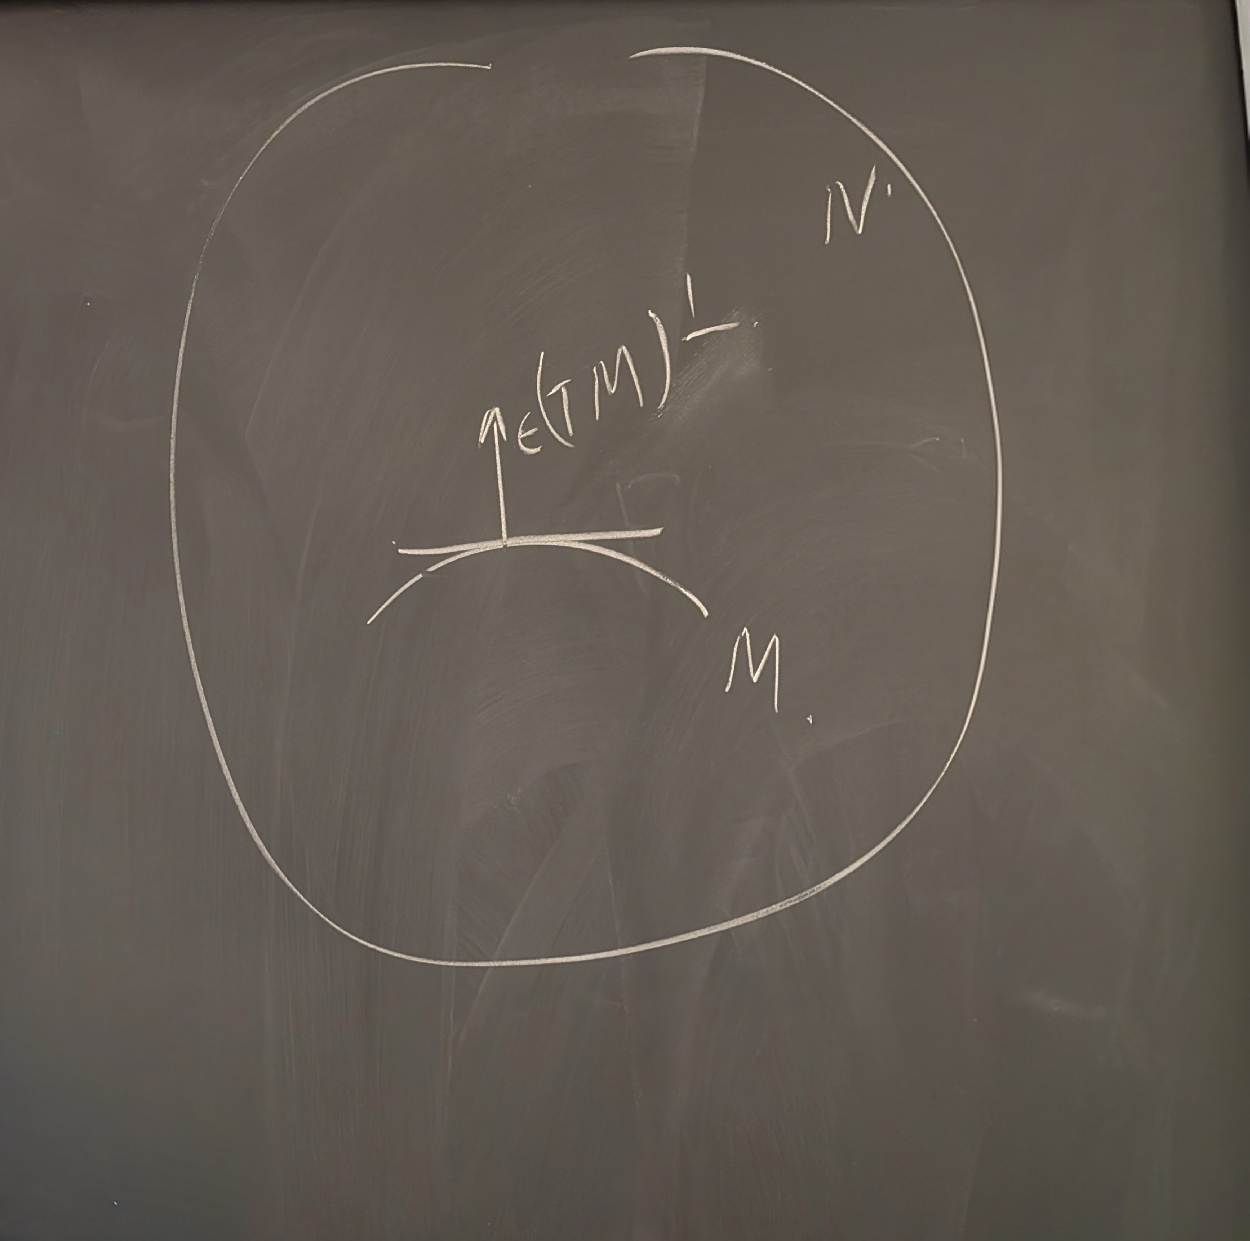
\includegraphics[width=0.4\textwidth]{img/normal}
            \caption{}
        \end{figure}

        If \(N \subset \mathbb{R}^k\) (or \(N\) Riemannian metric space) then \((TM)^\perp \subset \eval{TN}_{M}\).

        \[
            \begin{tikzcd}
                (TM)^\perp \ar[rr, bend right, "\cong"] \ar[r] & \eval{TN}_{M}^{} \ar[r] & \nu(M \hookrightarrow N) 
            \end{tikzcd}
        \]

        We have \((TN)_M = TM \oplus (TM)^\perp\).

        If \(\xi\) is a bundle with metric and \(\eta\) is a subbundle then \(\xi = \eta \oplus \eta^\perp\) and \(\eta^\perp \cong  \xi / \eta\).

    \end{enumerate}

    If \(B\) is paracompact [eg \(B \subset W\)] then bundles over \(B\) form an exact category [meaning all SES split].
    
    Reason: consider the following SES:

    \[
        0 \to \alpha  \to \beta \to \gamma \to 0
    \]

    Since \(B\) is paracompact we can give \(\beta\) a metric. \(\alpha^ \perp \xrightarrow{\approx} \gamma\) so it splits.
    
    This tells us: if \(M \subset N\) and \(N\) has a Riemannian metric, then,
    
    \(\eval{TN}_{M}^{} = TM \oplus TM^ \perp \cong TM \oplus \nu(M \hookrightarrow N)\).

    \begin{definition}
        Smooth \(f: M \to N\) is a immersion/submersion if \(\forall x\in M\), \(df_x\) is injective/surjective.
    \end{definition}

    For example, consider \(S^1 \to \mathbb{R}^2\) given by \(\bigcirc \to \infty\) is an immersion, since it's locally an embedding.

    \(TS^2 \to S^2\) is a submersion.

    Let \(f: M\to N\) be an immersion. Then, \(\nu(f) = \frac{f^{\ast} TN}{TM}\).

    If \(N\) has a metric then \(TM \cong \eval{TN}_{M}^{} \oplus \nu (f)\).

    \section*{Tuesday, 9/16/2025}

    \subsection*{UCT, Cup and Cap Prodcuts}
    
    Let \(M\) be an abelian group. Then we have homology \(H_i(X,A;M)\) and cohomology \(H^i(X,A;N)\) abelian groups.
    
    The cohomology \(H^i(X,A;N)\) is the cohomology of the following cochain complex: \(H^i(\operatorname{Hom} (S_\bullet(X,A),N))\) 

    `Cohomology eats homology' via the following \textit{Kronecker Pairing}:

    \[
        \langle , \rangle: H^i(X,A;N) \otimes H_i(X,A;M) \to N \otimes_\mathbb{Z} M
    \]

    \[
        [\phi] \otimes \left[ \sum_{i} k_i \sigma_i \otimes m_i \right] \mapsto \sum_{i} k_i \varphi (\sigma_i) \otimes m_i
    \]

    Now we do UCT. Let \(R = \mathbb{Z}\) and \(M = \mathbb{Z}\)-module, i.e. abelian group.
    
    If \(X = \mathbb{R} P^n\) then the cellular chain complex of \(\mathbb{R} P^n\) is:

    \[
        C_\bullet X = \mathbb{Z} \xrightarrow[0 \text{ \(n\) odd}]{2 \text{ \(n\) even}}\cdots \to \mathbb{Z} \xrightarrow{2} \mathbb{Z} \xrightarrow{0} \mathbb{Z}
    \]

    Thus, if \(n\) odd, then \(H_i \mathbb{R} P^n = \begin{dcases}
        \mathbb{Z} , &\text{ if } i = 0,n ;\\
        \mathbb{Z} _2, &\text{ if } i \text{ odd, } 0 < i < n ;\\
        0, &\text{ otherwise} .
    \end{dcases}\)

    If coefficients are in \(\mathbb{Z}_2\) then,
    
    \[
        C_\bullet X \otimes \mathbb{Z}_2 \xrightarrow{0} \mathbb{Z}_2 \xrightarrow{0} \cdots \xrightarrow{0} \mathbb{Z}_2
    \]

    Thus \(H_i (\mathbb{R} P^n;\mathbb{Z}_2) = \mathbb{Z}_2\) for \(0 \leq i \leq n\).

    UCT states that the following is a split short exact sequence:

    \[
        0 \to H_i X \otimes M \to H_i(X;M) \to \operatorname{Tor} (H_{i-1} X,M) \to 0
    \]

    We can say three things about Tor:

    Tor is a functor, \(\operatorname{Tor}: \operatorname{Ab} \times \operatorname{Ab} \to \operatorname{Ab}\).

    If \(M,N\) are f.g. then \(\operatorname{Tor} (M,N) \cong (\text{torsion } M) \otimes_\mathbb{Z} (\text{torsion } N)\) 

    \begin{definition}
        Find an exact sequence of free groups as follows:

        \[
            0 \to F_1 \to F_0 \to M \to 0
        \]

        Then \(\operatorname{Tor}(M,N) = H_1(F_1 \otimes N \to F_0 \otimes N)\).
    \end{definition}

    For example, \(\operatorname{Tor}(\mathbb{Z}_2, \mathbb{Z}_2)\), we have following free groups:

    \[
        0 \to \mathbb{Z} \xrightarrow{\times 2} \mathbb{Z} \xrightarrow{\text{mod } 2} \mathbb{Z}_2 \to 0
    \]

    Tensoring with \(\mathbb{Z}_2\) to get the following: \(\mathbb{Z}_2 \xrightarrow{0} \mathbb{Z}_2\). Then \(H_1\) is the kernel.

    So, \(\operatorname{Tor}(\mathbb{Z}_2, \mathbb{Z}_2) = \mathbb{Z}_2\).

    Now we go back to geometry.

    Suppose we have space \(X\) such that \(H_{i-1} X = \mathbb{Z}_2 \oplus ?\)

    This gives us \(H_i(X) \to \mathbb{Z}_2 \subset H_i(X;\mathbb{Z}_2)\).

    Geometrically, consider \(H_i(X;\mathbb{Z}_2) \to \operatorname{Tor}(H_{i-1} (X); \mathbb{Z}_2)\).
    
    If there is \([a] \in \operatorname{Tor}(H_{i-1} X; \mathbb{Z}_2)\) with \(2a = \partial b\) then section given by \([b] \mapsfrom [a]\)  

    UCT works even if we change \(\mathbb{Z}\) with a PID. For any PID \(R\) we can talk about \(R\)-modules \(M\), then \(H_i(X;M) \cong H_i(X;R) \otimes M \oplus \operatorname{Tor}^R(H_{i-1}(X;R),M)\).

    We want the analogue of UCT for cohomology. This gives us the split exact sequence:

    \[
        0 \to \operatorname{Ext}(H_{i-1} X, M) \to H^i(X;M) \to \operatorname{Hom}(H_i X, M) \to 0
    \] 

    Again, for \(n\) odd consider the chain complex:

    \[
        C_\bullet \mathbb{R} P^n = \mathbb{Z} \xrightarrow{0} \mathbb{Z} \to \cdots \mathbb{Z} \xrightarrow{2} \mathbb{Z} \xrightarrow{0} \mathbb{Z} \to 0
    \]

    For cochain complex we'd simply reverse the arrows:

    \[
        C^\bullet \mathbb{R} P^n = \mathbb{Z} \xleftarrow{0} \mathbb{Z} \leftarrow \cdots \mathbb{Z} \xleftarrow{2} \mathbb{Z} \xleftarrow{0} \mathbb{Z} \leftarrow 0
    \]

    \(H_i \mathbb{R}P^n = \mathbb{Z}\) for \(i=0,n\) and \(\mathbb{Z}_2\) for \(0 < i < n, n\) odd.

    \(H^i (\mathbb{R} P^n; \mathbb{Z} ) = \mathbb{Z}\) for \(i = 0,n\) and \(\mathbb{Z}_2\) for \(0 < i < n, n\) even.
    
    We have: \(\operatorname{Ext}(\text{Free}, M) = 0\).
    
    In general, \(\operatorname{Ext}(A,B)\) is given by: resolve \(A\), apply \(\operatorname{Hom}(-,B)\) cohomolgy.

    Suppose \(0 \to F_1 \to F_0 \to A \to 0\).

    Then, \(\operatorname{Hom}(F_1, B) \xleftarrow{\partial^1} \operatorname{Hom}(F_0, B)\).

    Thus \(\operatorname{Ext}(A,B) = \operatorname{coker} \partial^1\).

    If \(A, B\) are finitely generated then \(\operatorname{Ext}(A,B) \cong (\operatorname{torsion} A) \otimes B\).

    Now, suppose \(R\) is a commutative ring.

    Then \(H^i(X;R) = H^i(\operatorname{Hom}_\mathbb{Z}(X_\bullet X, R))\)
    
    But might be more in the spirit of how we are doing this to do the following:

    \(H^i(X;R) = H^i(\operatorname{Hom}_R(S_\bullet(X;R),R))\)
    
    For \(R\)-modules \(M\),

    \(H^i(X;M) = H^i(\operatorname{Hom}_\mathbb{Z}(S_\bullet X, M)) = H^i(\operatorname{Hom}_R(S_\bullet(X;R),M))\)
    
    Then, \(H^{\ast} (X;R)\) is a graded commutative ring under the cup product.

    \(H^{\ast} (X;R)\) is a graded commutative ring meaning we can write:
    
    \(H^{\ast} (X;R) = \bigoplus_{i \geq 0} H^i(X;R)\) and we have \(H^i(X;R) \otimes_R H^j(X;R) \to H^{i+j} (X;R)\)

    Commutative graded ring meaning \(\alpha \cup \beta = (-1)^{\vert \alpha  \vert \vert \beta \vert} \beta \cup \alpha\).
    
    For De Rham cohomology,

    \(H^i_{\text{DR}}(M;\mathbb{R}) \otimes H^j_{\text{DR}}(M;\mathbb{R})\) we have \(\alpha  \otimes \beta  \mapsto [\alpha \wedge \beta]\) 

    We also have: \(H_{\ast} (M;R)\) is a graded module over \(H^{\ast} (M;R)\) w.r.t.\ cap product.

    For \(\alpha \in H^i(M;R)\) and \(z\in H_j(M;R)\) then \(\alpha \cap z \in H_{j-i}(M;R)\).

    So, cap product by \(\alpha\) eats \(i\) dimensions from \(z\).

    We also have \(\langle \alpha \cup \beta, z \rangle = \langle \alpha , \beta \cap z \rangle \).

    If \(f: X\to Y\) is continuous, we have a ring map \(f^{\ast} : H^{\ast} (Y;R) \to H^{\ast} (X;R)\) by \(f^{\ast} (\alpha \cup \beta) = f^{\ast} \alpha \cup f^{\ast} \beta\).

    Poincar\'e Duality: if \(M^n\) is closed and oriented and connected then \(H_n M \cong \mathbb{Z}\). Choose generator \([M] \in H_n M\).

    Then we have isomorphism \(\cap [M]: H^i M \xrightarrow{\cong} H_{n-i} M  \) 

    Another fact:

    \[
        \frac{H^i M}{\text{torsion}} \otimes \frac{H^{n-i} M}{\text{torsion}} \to \mathbb{Z}
    \]

    is a nonsingular perfect pairing: \(\alpha \otimes \beta\) is given by \((\alpha \cup \beta)[M] \in \mathbb{Z}\).

    Recall \(A \times B \to \mathbb{Z}\) is perfect \(\iff A \xrightarrow{\cong} \operatorname{Hom}(B,\mathbb{Z})\) and \(B \xrightarrow{\cong} \operatorname{Hom}(A,\mathbb{Z})\) are isomorphism.

    In \(\mathbb{C} P^n = e^0 \cup e^2 \cup \cdots \cup e^{2n}\) we have \(H^{\ast} \mathbb{C} P^n \cong \mathbb{Z} [\alpha] / \alpha^{n+1}\), with \(\deg \alpha = 2\).

    This is a truncated polynomial ring.

    We can prove this by Poincar\'e duality and induction on \(n\).

    We also have Kunneth Theorem. If \(R\) is a field, then:

    \[
        H^{\ast} (X;R) \otimes H^{\ast} (Y;R) \xrightarrow{\cong} H^{\ast}(X \times Y; R)
    \]

    It is only an injection for general ring.

    \section*{Wednesday, 9/17/2025}
    
    HWK due 9/29.

    4 Exercises: 1 from Ch2, 1 from Ch3, 2 from Ch4.

    Today we finish chapter 3, construction of bundles.

    We skipped part f on Friday.

    \begin{table}[H]
        \centering
        \begin{tabular}{c|c}
            \toprule
                Vector Spaces & Vector Bundle \\
            \midrule
                \(V \otimes W\) & \(\xi \otimes \eta\) \\
                \(\operatorname{Hom}(V,W)\) & \(\operatorname{Hom}(\xi, \eta)\) \\
                \(V^{\ast} = \operatorname{Hom} (V,\mathbb{R})\) & \(\xi ^{\ast} = \operatorname{Hom} (\xi , \epsilon_B^1)\) \\
                \(\Lambda^k V\) & \(\Lambda ^k \xi\) \\
                \(\Lambda ^{\ast} V\) & \(\Lambda ^{\ast} \xi\)  \\
            \bottomrule
        \end{tabular}
        \caption{Anythong we can do on Vector Spaces, we can do in Vector Bundles.}
    \end{table}

    As for \(\operatorname{Hom}(\xi, \eta)\) we assume base space is the same:
    
    \[
        \begin{tikzcd}
            \operatorname{Hom}(\mathbb{R}^k, \mathbb{R}^l) \ar[r] & E \operatorname{Hom}(\overset{k}{\xi}, \overset{l}{\eta}) \ar[d] \\ & B
        \end{tikzcd}
    \]

    Here \(E \operatorname{Hom}(\xi, \eta) =\) [roughly] \(\bigcup_{b\in B} \operatorname{Hom}_{\mathbb{R}} (F_b(\xi), F_b(\eta))\)
    
    \(\coloneqq \coprod_{\text{open } U \subset B, \eval{\xi}_U, \eval{\eta}_U \text{ trivial}} U \times \operatorname{Hom}(\mathbb{R}^k, \mathbb{R}^l) / \sim\).
    
    \section*{Cotangent Bundle}

    Let \(M^n\) be a smooth \(n\)-manifold.

    \begin{definition}
        [Cotangent Bundle] Is dual to the tangent bundle: \(T^{\ast} M \coloneqq (TM)^{\ast}\).
    \end{definition}

    We can take exterior power to get differential \(k\) forms:

    \[
        \begin{tikzcd}
            \Lambda^k \mathbb{R} ^ n \ar[r] & \Lambda ^k T^{\ast} M \ar[d] \\ & M \ar[u, bend right, dotted]
        \end{tikzcd}
    \]

    Differential \(k\)-form on \(M, \omega \in \Gamma (\Lambda ^ k T^{\ast} M)\) smooth section.

    \(\begin{matrix}
        \Lambda ^{\ast} \mathbb{R}^n \to & \Lambda ^{\ast} T^{\ast} M \\
        & \downarrow \\
        & M \\
    \end{matrix} \leftarrow\) wedge product. 

    In fact, \(\Gamma (\Lambda ^{\ast} T^{\ast} M)\) is a graded algebra, \(\Omega ^{\ast} M\).
    
    \section*{Chapter 4}

    Now we start on Characteristic Classes.

    \begin{definition}
        [Stiefel-Whitney Classes] have these 4 axioms:

        \begin{enumerate}[label=\arabic*)]
            \item \(\forall\) vector bundle \(\xi\), assign \(\operatorname{w}_i(\xi) \in H^i(B(\xi);\mathbb{F}_2)\) so that \(\operatorname{w}_0(\xi) = 1\) and \(\operatorname{w}_i(\xi) = 0\) for \(i > n\) when \(\xi\) is a an \(n\)-plane bundle.
            \item \textit{Naturality}: For continuous \(f: B^{\prime} \to B(\xi)\), we have \(\operatorname{w}_i(f^{\ast} \xi) = f^{\ast} (\operatorname{w}_i \xi) \in H^i(B;\mathbb{F}_2)\). [First one is the pullback on the bundle, second one is the induced map on the cohomology.]
            \item \textit{Whitney Sum Formula}: If \(\xi , \eta\) are vector bundles over \(B\) we have: \(\operatorname{w}_k(\xi \oplus \eta) = \sum_{i+j=k} \operatorname{w}_i(\xi) \cup \operatorname{w}_j(\eta) \).
            \item \(0 \neq \operatorname{w}_1(\gamma^1_1) \in H^1(P^1;\mathbb{F}_2) = H^1(S^1; \mathbb{F}_2) = \mathbb{F}_2\).
        \end{enumerate} 

        This sequence of cohomology classes is called the Stiefel-Whitney Classes.

    \end{definition}

    Recall: \(\gamma^1_1\) for a mobius strip is the zero section, i.e. \(S^1\).

    Milnor-Stasheff says naturality a bit differently. Recall: If

    \[
        \begin{tikzcd}
            E(\eta) \ar[r, "\text{iso/fibers}"] \ar[d] & E(\xi) \ar[d] \\ B(\eta) \ar[r,"f"] & B(\xi)
        \end{tikzcd}
    \]

    then \(\eta = f^{\ast} \xi, \operatorname{w}_i(\eta) = f^{\ast} \operatorname{w}_i(\xi)\).

    Note: axioms 1 and 2 says \(\operatorname{w}_i\) are \textit{characteristic classes}. Characteristic Classes are cohomology classes respecting naturality. Meaning they respect nontriviality of bundles. Just like homology `classifies' upto homotopy in a sense, we need characteristic classes to capture the `twists' in a vector bundle.

    Axiom 1 and 2 implies:

    \begin{proposition}
        [1] \(\xi \cong \eta \implies \operatorname{w}_i(\xi) = \operatorname{w}_i(\eta)\).
    \end{proposition}

    Recall that vector bundles are isomorphic if:

    \[
        \begin{tikzcd}
            E(\xi) \ar[rr,"\cong"] \ar[rd] & & E(\eta) \ar[dl] \\ & B
        \end{tikzcd}
    \]

    \begin{proof}
        \(f = \operatorname{id}\).
    \end{proof}

    \begin{proposition}
        [2] \(\operatorname{w}_i(\epsilon^n_B) = 0\) for \(i > 0\).  
    \end{proposition}

    \begin{proof}
        \[
            \begin{tikzcd}
                B \times \mathbb{R}^n \ar[r] \ar[d] & \mathbb{R}^n \ar[d] \\ B \ar[r,"c"] & \text{pt}
            \end{tikzcd}
        \]

        \(\operatorname{w}_i(\epsilon^n_B) = \operatorname{w}_i (c^{\ast} \epsilon^n_{\text{pt}}) = c^{\ast} \operatorname{w}_i(\epsilon^n_{\text{pt}}) \in H^i(\text{pt};\mathbb{F}_2) = 0\).
        
        Thus, nontrivial Stiefel-Whitney Class implies nontrivial bundle.

    \end{proof}

    \begin{proposition}
        [3] If \(\epsilon\) trivial then \(\operatorname{w}_i(\epsilon \oplus \eta) = \operatorname{w}_i(\eta)\). In other words, \(\operatorname{w}_i\) stable characteristic classes.
    \end{proposition}

    \begin{proposition}
        [4] If \(\xi\) is an \(n\)-plane bundle with \(k\) linearly independent sections, then \(k\) of them vanishes:

        \[
            \operatorname{w}_{n-k+1}(\xi) = \cdots = \operatorname{w}_{n-1} (\xi) = \operatorname{w}_n(\xi) = 0
        \]
    \end{proposition}

    Most interesting case is \(k = 1\) contrapositive.

    \(\operatorname{w}_n(\xi) \neq 0 \implies \not\exists\) nowhere zero section. Hairy ball theorem!

    eg for \(n\) odd there exists a nowhere zero section of the tangent bundle \(TS^n\). Therefore, \(\operatorname{w}_n(TS^n) = 0\).
    
    Since \(n\) is odd \(n+1\) is even, and we can switch the coordiantes in pairs:

    \[
        \underline{x} = (x_1, \cdots , x_n) \mapsto (\underline{x}, -x_2, x_1, \cdots ,-x_{n+1}, x_n) \in TS^n \subset S^n \times \mathbb{R}^{n+1} 
    \]

    \(\operatorname{w}_4(T \mathbb{C} P^2)\neq 0, \not\exists\) nowhere vanishing vector field on \(\mathbb{C}P^2\).

    If \(M^n\) is a closed \(n\)-manifold then \(\operatorname{w}_n(TM^n) \equiv \xi(M) \pmod 2\).

    \begin{proof}
        The condition of \(k\) linearly independent section is equivalent to existence of a subbundle \(\epsilon^k_B \subset \xi\).

        Case 1: Suppose \(\xi\) has a metric.

        Then \(\xi = \epsilon^k_B \oplus (\epsilon^k_B)^{\perp}\). 

        \(\operatorname{w}_i(\xi) = \operatorname{w}_i(\epsilon^{k \perp}_B)\) by proposition 3. Note that \(\epsilon^{k \perp}_B\) is a \(n - k\) bundle, axiom 1 implies the statement.

        Case 2: \(B\) is a CW complex so \(B\) is paracompact which implies \(\xi\) has a metric.

        General case: suppose \(\begin{matrix} E(\xi) \\ \downarrow \\ B \end{matrix}\). Then \(\exists\) CW-approximation \(B^{\prime} \to B\) where \(B^{\prime}\) is a CW complex which is isomorphism on \(\pi_{\ast}\) which is isomorphism in homology and cohomology. This reduces to case 2.

    \end{proof} 

    \section*{Friday, 9/19/2025}
    
    Recap: Stiefel-Whitney-Classes:

    Suppose we have an \(n\)-plane bundle \(\begin{pmatrix}
        \mathbb{R}^n & \to & E \\
         &  & \downarrow \\
         &  & B \\
    \end{pmatrix} \) 

    Then \(\operatorname{w}_i E = \operatorname{w}_i (\xi) \in H^i(B;\mathbb{F}_2)\).

    We have some axioms:

    \begin{enumerate}[label=\arabic*)]
        \item \(\operatorname{w}_0(\xi) = 1, \operatorname{w}_i(\xi) = 0\) for \(i > n\)
        \item Naturality: if we have \(f: B^{\prime} \to B\) then \(\operatorname{w}_i(f^{\ast} \xi) = f^{\ast} \operatorname{w}_i(\xi) \in H^i(B^{\prime} ; \mathbb{F}_2)\).
        
        One way to rephrase it is as follows: \(f^{\ast} E\) is the pullback bundle in the following:

        \[
            \begin{tikzcd}
                f^{\ast} E \ar[r] \ar[d] & E \ar[d] \\ B^{\prime} \ar[r,"f"] & B
            \end{tikzcd}
        \]

        Another way: if we have a bundle map:

        \[
            \begin{tikzcd}
                E^{\prime} \ar[r] \ar[d] & E \ar[d] \\ B^{\prime} \ar[r] & B
            \end{tikzcd}
        \]

        which is an isomorphism on the fibers, then \(f^{\ast} E \cong E^{\prime}\). We have \(E^{\prime} \to B^{\prime} \) which is equal to \(f^{\ast} \xi\).

        In Milnor-Stasheff, if we have:

        \[
            \begin{tikzcd}
                E(\eta) \ar[r] \ar[d] & E(\xi) \ar[d] \\ B(\eta) \ar[r] & B(\xi)
            \end{tikzcd}
        \]

        \(\eta \to \xi\) in this case \(\operatorname{w}_i(\eta) = f^{\ast} \operatorname{w}_i(\xi)\).

        Note that properties 1 and 2 are called characteristic class on a bundle.

        \item Whitney Sum formula: \(\operatorname{w}_k(\xi \oplus \eta) = \sum_{i+j=k} \operatorname{w}_i(\xi) \operatorname{w}_i(\eta)\)
        \item \(\operatorname{w}_1(\gamma^1_1) \neq 0\).
    \end{enumerate} 

    Recall proposition 3: if \(\epsilon\) trivial then \(\operatorname{w}_i(\epsilon \oplus \eta) = \operatorname{w}_i(\eta)\).

    Proposition 4: \textit{obstruction to sections}: If \(\xi\) has \(k\)-linearly independent sections then the top \(k\) Stiefel-Whitney Classes vanish.

    \subsection*{Whitney Sum Inverses}

    \begin{definition}
        Suppose \(\xi \oplus \eta = \epsilon^N\). Then \(\xi\) and \(\eta\) are whitney sum inverses of each other.
        
        Example: Normal bundle and tangent bundle.
    \end{definition}

    Fact: \(\dim B < \infty\) implies every bundle has an inverse.

    Observation: \(\operatorname{w}_{\ast} (\xi)\) can be computed in terms of \(\operatorname{w}_{\ast} (\eta)\).

    \[
        0 = \operatorname{w}_1(\xi \oplus \eta) = \operatorname{w}_1(\xi) + \operatorname{w}_1 (\eta) \implies \operatorname{w}_1(\xi) = \operatorname{w}_1(\eta)
    \]
    
    \[
        0 = \operatorname{w}_2(\xi \oplus \eta) = \operatorname{w}_2(\xi) + \operatorname{w}_1(\xi) \operatorname{w}_1(\eta) + \operatorname{w}_2(\eta) \implies \operatorname{w}_2(\xi) = \operatorname{w}_1(\eta)^2 + \operatorname{w}_2(\eta)
    \]

    In Milnor Stasheff, they define a new ring:

    \[
        H^{\prod}  (B;\mathbb{F}_2) = \prod_i H^i(B;\mathbb{F}_2)
    \]

    This allows us to take infinite series:

    \[
        \operatorname{w}(\xi) = 1 + \operatorname{w}_1 \xi + \operatorname{w}_2 \xi + \cdots \in H^{\prod}  (B;\mathbb{F}_2)
    \]

    Then we can rephrase the Whitney sum theorem as follows:

    \(\operatorname{w}(\xi \oplus \eta) = \operatorname{w}(\xi) \cup w(\eta)\).

    \begin{lemma}
        \(\left\{ 1 + a_1 + a_2 + \cdots \in H^{\prod} (B;\mathbb{F}_2) \mid a_i \in H^i(B;\mathbb{F}_2) \right\}\)
    \end{lemma}

    \begin{proof}
        Due to `Euler':

        \((1 + a_1 + a_2 + \cdots ) ^{-1}  = \frac{1}{1+(a_1 + a_2 + \cdots)}\)
        
        \(= 1 + (a_1 + a_2 + \cdots ) + (a_1 + a_2 + \cdots)^2 + (a_1 + a_2 + \cdots)^3\)

        \(= 1 + a_1 + (a_2 + a_1^2) + (a_3 + a_1^3) + \cdots\) 
        
        
    \end{proof}

    Notation: Suppose \(\operatorname{w}(\xi) \in H^{\prod} (B;\mathbb{F}_2)\) then we can have the formal multiplicative inverse: \(\overline{\operatorname{w}}(\xi) \in H^{\prod } (B;\mathbb{F}_2)\) so that \(\operatorname{w} (\xi) \overline{\operatorname{w}}(\xi) = 1\)  

    This gives us the following observation: \(\xi \oplus \eta = \epsilon^N\) gives us \(\operatorname{w}(\xi) \operatorname{w}(\eta) = 1 \implies \operatorname{w}(\xi) = \overline{\operatorname{w}}(\eta)\).
    
    eg \(H^{\ast} (\mathbb{P}^{\infty} ;\mathbb{F}_2) = \mathbb{F}_2[a]\) then we have canonical line bundle \(\gamma^1\) then \(\operatorname{w} (\gamma^1) = 1+a\) so \((1+a)^{-1} = 1 + a + a^2 + \cdots\) which has infinitely many terms so the inverse might not exist! The line bundle doesn't have any whitney sum inverse.

    \begin{theorem}
        [Whitney Duality Theorem] Let \(M^n \subset \mathbb{R} ^N\) be a smooth manifold. Then \(\operatorname{w}_i(TM) = \overline{\operatorname{w}}_i \left( \nu (M \hookrightarrow \mathbb{R}^N) \right)  \) 
    \end{theorem}

    \begin{proof}
        \((TM \oplus \nu (M \hookrightarrow \mathbb{R}^N)) = \eval{T\mathbb{R}^N}_M\) 
    \end{proof}

    \begin{lemma}
        Suppose we have a closed codim \(1\) manifold: \(M^n \subset \mathbb{R}^{n+1}\). Then \(\operatorname{w} (TM) = 1\).
    \end{lemma}

    So Stiefel-Whitney Classes give an obstruction to submanifolds of codimension \(1\).

    \begin{proof}
        \(TM \oplus \nu (M \hookrightarrow \mathbb{R}^{n+1})\) is trivial, \(\nu (M \hookrightarrow \mathbb{R}^{n+1})\) gives nowhere zero section.
    \end{proof}

    \begin{corollary}
        Non-orientable submanifolds must have codimension at least \(2\).
    \end{corollary}

    Recall \(P^n = \mathbb{R} P^n = S^n / x \sim -x = \frac{S^n_+}{x \sim -x \text{ when } x \in S^{n-1}} =\) lines in \(\mathbb{R}^{n+1}\) through \(0\).
    
    \(P^n\) is a CW complex via the pushout:

    \[
        \begin{tikzcd}
            S^{n-1} \ar[r] \ar[d, hook] & P^{n-1} \ar[d] \\ D^n \ar[r] & P^n
        \end{tikzcd}
    \]

    \(P^0 \subset P^1 \subset \cdots \subset P^n\) is the skeleton.

    Essentially \(P^n = e^0 \cup e^1 \cup \cdots \cup e^n\) with \(e^i \cong \overset{\circ}{D^i}\).
    
    Cellular chain complex:

    \[
        C_\bullet(P^n; \mathbb{F}_2) = \mathbb{F}_2 \xrightarrow{0} \cdots \xrightarrow{0} \mathbb{F}_2
    \]

    Cochain complex:

    \[
        C^\bullet(P^n;\mathbb{F}_2) = \mathbb{F}_2 \leftarrow \cdots \leftarrow \mathbb{F}_2
    \]

    \(H_{\ast} (P^n;\mathbb{F}_2) = H^{\ast} (P;\mathbb{F}_2) = \{ \mathbb{F}_2: x \leq n \}\)

    Next: \(H^{\ast} (P^n;\mathbb{F}_2) = \frac{\mathbb{F}_2[a]}{a^{n+1}}\) truncated polynomial ring. 

    \section*{Monday, 9/22/2025}
    
    We do some computations today.

    Recall: \(P^n = S^n / x \sim -x = \underbrace{e^0 \cup e^1 \cup \cdots}_{P^{n-1} } \cup e^n\)

    Then \(H^{\ast} (P^n; \mathbb{F}_2) = \begin{dcases}
        \mathbb{F}_2, &\text{ if } \ast \leq n ;\\
        0, &\text{ otherwise} .
    \end{dcases}\) 

    Let \(0 \neq a \in H^1(P^n; \mathbb{F}_2)\).

    \begin{theorem}
        \(H^{\ast} (P^n; \mathbb{F}_2) = \frac{\mathbb{F}_2[a]}{a^{n+1}}\), truncated polynomial ring.
    \end{theorem}

    \begin{proof}
        Induction on \(n\) and Poincar\'e Duality.

        It is true for \(n = 1\).

        Now suppose it is true for \(n - 1\).

        We have injection \(i : P^{n-1} \hookrightarrow P^n\). Thus \(i^{\ast}\) is a ring map isomorphism on dimension \(\leq n - 1\).

        Thus \(a, a^2, \cdots , a^{n-1}\) non-zero.

        Question: do we have \(a^n \neq 0\)?
        
        We use Poincar\'e Duality to prove that.

        Suppose \([P^n] \in H_n(P^n;\mathbb{F}_2) \neq 0\).
        
        Then we have: \(\cap [P^n]: H^{n-1} (P^n;\mathbb{F}_2) \xrightarrow{\sim} H_1(P^n;\mathbb{F}_2)\).
        
        Then \(\langle a^n, [P^n] \rangle = \langle a^{n-1}, a\cap [P^n] \rangle \neq 0\) since UCT implies:
        
        \(H^{n-1}(P^n;\mathbb{F}_2) \xrightarrow{\approx} \operatorname{Hom} (H_{n-1}(P^n;\mathbb{F}_2),\mathbb{F}_2)\) by \(\beta \mapsto (b \mapsto \langle \beta , b \rangle )\) and both \(a^{n-1}\) and \(a\cap [P^n]\) are nonzero.
    \end{proof}

    Now we can look at SW classses of \(\gamma_n^1\) and \(TP^n\).

    \begin{proposition}
        \(\operatorname{w} (\gamma_n^1) = 1 + a \in H^{\ast} (P^n; \mathbb{F}_2)\).
    \end{proposition}

    \begin{proof}
        True for \(n=1\) by axiom \(4\).

        Now consider restriction: \(\eval{\gamma^1_n}_{P^1} = \gamma^1_1\).

        By the axiom we have \(1+a = \operatorname{w}(\gamma^1_1) = i^{\ast} \operatorname{w} (\gamma^1_n)\).
    \end{proof}

    Now let \(\gamma=\gamma^1_n = \left\{ \{ ([x],v) \} \mid v\in \mathbb{R}x \right\} \subset P^n \times \mathbb{R}^{n+1}\) be the tautological line bundle.

    \(\gamma \subset \epsilon^{n+1}_{P^n} \implies \gamma \oplus \gamma^{\perp} =\epsilon^{n+1} \).

    Therefore, \(\operatorname{w}(\gamma^{\perp}) = \overline{\operatorname{w}}(\gamma) = (1+a)^{-1} = 1 + a + \cdots + a^n \in H^{\ast} (P^n;\mathbb{F}_2)\). 

    Thus \(\gamma^{\perp}\) has no nonzero sections.

    \begin{corollary}
        \(\gamma^1_\infty\) over \(P^{\infty}\) has no W.SI.
    \end{corollary}

    Question: \(\operatorname{w}(TP^n) = ?\) 

    Recall: \(G \curvearrowright X\) then orbit space \(X / G = X / x \sim gx, S^n / C_2 = P^n\).

    \begin{theorem}
        \begin{enumerate}[label=\roman*)]
            \item \(TP^n \oplus \epsilon^1 = \underbrace{\gamma \oplus \cdots \oplus \gamma}_{n+1}\).
            \item \(\operatorname{w} (TP^n) = (1+a)^{n+1} = \sum_{j=0}^n \binom{n+1}{j} a^j \in H^{\ast} (P^n;\mathbb{F}_2) \)
        \end{enumerate} 
    \end{theorem}

    \begin{proof}
        Apply the antipodal map to:

        \[
            TS^n \oplus \nu = \epsilon^{n+1} = \epsilon ^1 \oplus \cdots \oplus \epsilon^1 \tag{\(\ast\)}
        \]

        To get the following:

        \[
            TP^n \oplus \epsilon = \gamma \oplus \cdots \gamma \tag{\(\ast \ast\)}
        \]

        where \(C_2 \curvearrowright S^n \times \mathbb{R}^{n+1}\) by \((x,v) \mapsto (-x,-v)\).

        Note: \(TP^n = (TS^n) / C_2\) since \(S^n\) is a covering space of \(TP^n\).

        Note: \(\nu(S^n \hookrightarrow \mathbb{R}^{n+1}) \cong \epsilon^1_{S^n}\)
        
        Note: \(\nu(S^n \hookrightarrow \mathbb{R}^{n+1}) / C_2 \cong \epsilon^1_{P^n}\)
        
        Note: \(\epsilon^1_{S^n} / C_2 \cong \gamma\) since \(\frac{S^n \times \mathbb{R}}{C_2} \cong E(\gamma)\) by \([(x,t)] \mapsto ([x],tx)\) 

        This proves \((\ast \ast)\).

        Now we prove i \(\implies\) ii.

        \(\operatorname{w}(P^n) = \operatorname{w}(TP^n \oplus \epsilon) = \operatorname{w}((n+1)\gamma) = \operatorname{w}(\gamma)^{n+1} = (1+a)^{n+1}\) 

    \end{proof}

    MS shows \(TP^n \cong \operatorname{Hom} (\gamma , \gamma^{\perp})\).

    \subsection*{Parallelizable Manifolds}
    
    \begin{definition}
        A manifold \(M^n\) is \textit{parallelizable} if \(TM^n = \epsilon^n_M \) [i.e. if there exists \(n\) linearly independent vector fields]
    \end{definition}

    eg \(S^{2n}\) is not parallelizable via the hairy ball theorem.

    Lie Groups are parallelizable: note that \(T_e G^n\) has basis \(e_1, \cdots , e_n\), and for \(g\in G\) we have \(\ell_g: G \to G\) given by \(h \mapsto gh\).

    We then have \(g \mapsto (d \ell_{g \ast})(e_i)\) giving \(n\) linearly independent vector fields. 

    Thus, \(\operatorname{w}_i(TM^n) \neq 0\) for \(i > 0\) implies \(M\) is not a lie group.

    \(S^0, S^1, S^3, P^0, P^1, P^3 (=\operatorname{SO}(3))\) are lie groups.

    \section*{Wednesday, 9/24/2025}
    
    \begin{corollary}
        [4.6i] \(\operatorname{w}_n(P^n) \neq 0 \iff n\) even.

        (ii). \(\operatorname{w}(P^n) = 1 \iff n+1 = 2^r\)
    \end{corollary}

    \begin{corollary}
        \(n\) even implies \(P^n\) has no nowhere zero vector field.

        \(P^n\) parallelizable [i.e. \(TP^n\) trivial] implies \(n = 2^r - 1\). 
    \end{corollary}

    \begin{proof}
        4.6i: \(\operatorname{w}_n(P^n) \neq 0 \iff \binom{n+1}{n}a^n \neq 0 \iff n+1 \neq 0 \iff n+1\) odd.

        4.6ii: \(\operatorname{w}(P^{2^r - 1}) = (1+a)^{2^r} = 1 + a^{2^r} = 1\) gives one direction. For other direction, if \(n+1 = 2^r m\) for odd \(m > 1\) then \(\operatorname{w}(P^n) = (1+a)^{2^r m} = (1 + a^{2^r})^m = 1 + m a^{2^r} + \cdots\).

    \end{proof}

    \begin{theorem}
        [4.7 Stiefel] Suppose \(\exists\) bilinear map \(p: \mathbb{R}^n \times \mathbb{R}^n \to \mathbb{R}^n\) without zero divisor [meaning \(p(x,y) = 0 \implies x=0\) or \(y=0\)].

        Then \(P^{n-1}\) is parallelizabl [thus \(n = 2^r\)].
    \end{theorem}

    e.g. \(\mathbb{R}, \mathbb{C} ,\mathbb{H} , \mathbb{O}\). Theorem by Adams states \(n = 1,2,4,8\).

    \begin{proof}
        Let \(\{ b_1, \cdots , b_n \} \) be basis for \(\mathbb{R}^n\). Define \(v_i\):

        \[
            \begin{tikzcd}
                \mathbb{R}^n \ar[rr, bend right, "v_i"] & \mathbb{R}^n \ar[l, "{p(-,b_1)}", swap] \ar[r, "{p(-,b_i)}"] & \mathbb{R}^n
            \end{tikzcd}
        \]

        Then \(x\neq 0 \implies p(x,b_1),\cdots ,p(x,b_n)\) are linearly independent, thus \(v_1(x), \cdots , v_n(x)\) linearly independent.

        Note that \(v_1(x) = x\).

        Define linearly independent sections \(s_2, \cdots , s_n\) of \(TP^{n-1}\).

        \(s_i[x] = [x,  \operatorname{pr}_{(\mathbb{R} x)^{\perp}}(v_i(x))]\in TP^{n-1} = (TS^{n-1}) / C_2\). 
    \end{proof}

    \section*{Stiefel-Whitney Numbers}

    We want to prove the following theorem:

    \begin{theorem}
        A closed manifold is a boundary \(\iff\) Stiefel-Whitney numbers are all zero.
    \end{theorem}

    We need to talk about first fundamental class.

    If \(M^n\) is a closed connected manifold [since we have \(\mathbb{F}_2\) coefficient we don't worry about orientation] then the fundamental class \([M] \in H_n(M;\mathbb{F}_2) \cong H^0(M;\mathbb{F}_2) = \mathbb{F}_2\).

    We dont really need connectedness. If \(M^n = M_1 \sqcup \cdots \sqcup M_k\) where each \(M_j\) are connected then the fundamental class \([M] = i_{1 \ast} [M_1] + \cdots + i_{k \ast} [M_k] \in H_n(M;\mathbb{F}_2) = \mathbb{F}_2^k\).

    \begin{definition}
        A partitition of \(n\) is \(r_1, \cdots , r_n \in \mathbb{Z}_{\geq 0}\) such that \(r_1 + 2r_2 + 3r_3 + \cdots + nr_n = n\).

        Let \(\Pi(n) =\) set of partitions of \(n\).

        For example, \(\Pi(4) = \left\{ (0,0,0,1),(0,2,0,0),(1,0,1,0),(2,1,0,0),(4,0,0,0)\right\} \) 
    \end{definition}

    \begin{definition}
        [Stiefel-Whitney Number] Given \((r_i) \in \Pi(n)\) the Stiefel-Whitney Number is defined by:

        \[
            \operatorname{w}_1^{r_1} \cdots \operatorname{w_n}^{r_n} [M] \coloneqq \left\langle \operatorname{w}_1(TM)^{r_1} \cup \cdots \operatorname{w}_n(TM)^{r_n}, [M] \right\rangle \in \mathbb{F}_2
        \]
    \end{definition}

    For example we find Stiefel-Whitney numbers of \(P^2\).

    \(\operatorname{w}(P^2) = \operatorname{w}(TP^2) = (1+a)^3 = 1+a+a^2\).

    \(\operatorname{w}_1^2 [P^2] = \langle a^2, P^2 \rangle = 1\) 

    \(\operatorname{w}_2 [P^2] = \langle a^2, P^2 \rangle = 1\)

    Thus \(P^2\) is not the boundary of a \(3\)-manifold.

    We can see this more easily since the characteristic of \(P^2\) is odd.

    \section*{Friday, 9/26/2025}
    
    Homeowork Due Monday.

    Ch2: 1 Exercise
    Ch3: 1 Exercise
    Ch4: 2 Exercise

    \section*{Manifolds with Boundary}

    Classic examples: disk \(D^n\), cylinder \(S^{n-1} \times I\)

    \begin{definition}
        \textit{Local Model} is the upper half-space \(H^n = \left\{ (x_1, \cdots , x_n) \in \mathbb{R}^n \mid x_1 \geq c \right\} \).
    \end{definition}

    \begin{definition}
        Let \(M \subset \mathbb{R}^A\). An \(n\)-\textit{manifold with boundary} such that \(\forall x\in M, \exists\) smooth homeomorphism (parameterization) \(h: V \to U\) where \(V \subset H^n\) and \(x \in U \subset M\) open such that \(\forall y\in V, \mathrm{d}h_y:\mathbb{R}^n \to \mathbb{R}^A\) has rank \(n\).
    \end{definition}

    \begin{definition}
        \(\operatorname{Int} M \coloneqq \left\{ x\in M \mid \exists \text{nbhd } U \cong \mathbb{R}^n \right\} \).
        
        \(\partial M \coloneqq M - \operatorname{Int} M\)

        \(M = \partial M \cup \operatorname{Int} M\) 
        
        \(D^n = S^{n-1} \cup \operatorname{Int} D^n\)
    \end{definition}

    \(n\)-manifold is \(n\)-manifold with boundary.

    manifold with nonempty interior is not a manifold.

    \(M\) is an \(n\)-manifold with boundary \(\implies \operatorname{Int} M\) is a \(n\)-manifold and \(\partial M\) is a \(n-1\) manifold.

    \(M \simeq \operatorname{Int} M\).

    Now consider tangent space:

    \(\begin{matrix}
        \mathbb{R}^n & \rightarrow & TM & = \{ (x,v) \mid x\in M, v= \gamma^{\prime} (0), \gamma(0)=x  \\ & & \downarrow & , \gamma : [0,\infty) \to M \lor \gamma :(-\infty,0] \to M \} \\ & & M
    \end{matrix}\) 

    Then \(\eval{TM}_{\partial} \cong T \partial M \oplus \epsilon^1\) where \(\epsilon^1\) is the outward poinitng normal, the nowhere zero section of \(\eval{TM}_\partial \).

    \subsection*{Poincar\'e-Lefschetz Duality}

    (PL duality).

    \begin{theorem}
        \(H_n(M, \partial M; \mathbb{F}_2) = \mathbb{F}_2\).
    \end{theorem}

    \begin{definition}
        Fundamental class \([M] \in H_n(M, \partial M; \mathbb{F}_2)\).
    \end{definition}

    \begin{theorem}
        [PL Duality]  \(\cap [M]: H^i(M, \partial M; \mathbb{F}_2) \xrightarrow{\approx} H_{n-i} (M;\mathbb{F}_2)\).

        \(\cap [M]: H^i(M,\mathbb{F}_2) \xrightarrow{\approx} H_{n-i} (M, \partial M, \mathbb{F}_2)\).
    \end{theorem}

    Exercise: Work this out for \(D^n\).

    Furthermore, if we look at the long exact sequence of a pair:

    \[
        H_n(M, \partial M; \mathbb{F}_2) \xrightarrow{\partial} H_{n-1}(\partial M;\mathbb{F}_2) \to H_{n-1}(M;\mathbb{F}_2)  
    \]

    then \(\partial [M] = [\partial M]\).

    \begin{theorem}
        [MS 4.9, Pontryagin] Suppose \(M\) is a compact \(n+1\)-manifold with boundary. Then the Stiefel Whitney numbers of \(\partial M\) are \(0\).
    \end{theorem}

    \begin{proof}
        WLOG \(M\) is connected. Let \(r_i \in \Pi(n)\) [thus \(\sum_{i} r_i i = n\)].

        Then \(\left\langle \operatorname{w}_1 (T \partial M)^{r_1} \cup \cdots \operatorname{w}_n(T \partial M)^{r_n}, [\partial M] (= \partial [M]) \right\rangle\)
        
        \(= \left\langle \delta (\operatorname{w}_1(T \partial M)^{r_1} \cdots \operatorname{w}_n(T \partial M)^{r_n}), [M] \right\rangle \).

        Now, recall:
    
        \[
            H^n(M;\mathbb{F}_2) \xrightarrow{i^{\ast}} H^n(\partial M, \mathbb{F}_2) \xrightarrow{\delta} H^{n+1} (M, \partial M; \mathbb{F}_2)
        \]

        WTS: \(\operatorname{w}_1(T \partial M)^{r_1} \cdots \operatorname{w}_n(T \partial M)^{r_n} \in \operatorname{im} i^{\ast}\).

        Note that it is equal to:

        \[
            \operatorname{w}_1 \left( i^{\ast} (TM) \right)^{r_1} \cdots \operatorname{w}_n(i^{\ast} (TM))^{r_n} = i^{\ast} \left( \operatorname{w}_1(TM)^{r_1} \cdots \operatorname{w}_n(TM)^{r_n} \right)  
        \]

    \end{proof}

    \begin{theorem}
        [P-Thom] A closed \(n\)-manifold is the boundary of a compact \(n\)-manifold iff all Stiefel Whitney numbers vanish.
    \end{theorem}

    Note that all manifolds are boundary of a not necessarily compact manifold, just take \(M \times [0,\infty)\) 

    \begin{definition}
        [Bordism Groups] Two closed \(n\)-dimenstional manifolds \(M_1, M_2\) are \textit{bordant} if \(\exists\) a compact \(W^{n+1}\) manifold with boundary such that \(\partial W \underset{\text{diff}}{\cong} M_1 \coprod M_2\). W is called the \textit{cobordism}.

        Easy exercise: Bordism is an equivalence relation. Canonical example: Pant \(\implies S^1 \sim S^1 \coprod S^1\).

        One can get a group \(\Omega^o_n = (\text{bordism classes of closed \(n\)-manifold}, \coprod)\).
        
        This is called the unoriented bordism group.

    \end{definition}

    Note that \(2 \Omega^o_n = 0\) since \(\partial (M \times I) = M \coprod M\), \(-[M] = [M]\).

    \begin{theorem}
        [Collar Neighborhood] \(\exists\) neighborhood \(U\) of \(\partial W\) and a diffeomorphism \(h: U \xrightarrow{i} \partial W \times [0,\infty)\) such that \(h(x,0)\) for \(x\in \partial W\).
    \end{theorem}

    Note that \(\Omega^o_{\ast}\) is a graded ring with cartesian product.

    \begin{table}[H]
        \centering
        \begin{tabular}{c|c|c}
            \toprule
                \(n\) & \(\Omega^n_o\) & \(\Pi(n)\) \\
            \midrule
                \(0\) & \(\mathbb{Z} / 2\) pt & \(1\) \\
                \(1\) & \(0\) & \(1\) \\
                \(2\) & \(\mathbb{Z}/2\, P^2\) & \(2\) \\
                \(3\) & \(0\) & \(0\) \\
                \(4\) & \(\mathbb{Z}/2 \oplus \mathbb{Z}/2\, P^4, P^2 \times P^2\) & \(5\) \\
                \(5\) & \(\mathbb{Z} / 2\) Wu-\(n\)-manifold \(SU(3) / SO(3)\) & \(7\) \\
            \bottomrule
        \end{tabular}
        \caption{Bordism Group Calculations}
    \end{table}

    \begin{theorem}
        [PT Theorem]

        \[
            \Omega^o_n \overset{\text{SW\#}}{\rightarrowtail} (\mathbb{F}_2)^{\Pi(n)}
        \]
    \end{theorem}

    \section*{Monday, 9/29/2025}
    
    Applications:

    Let \(M \to \overline{M}\) is a \(k\) to \(1\) covering map with \(k\) odd. Then,

    \(0 = [M]\in \Omega^o_n \iff 0 = [\overline{M}] \in \Omega^o_n\) 

    eg Lens spaces \(L(k)\) with \(k\) odd are boundaries.

    \begin{proof}
        \(H_n(M;\mathbb{F}_2) \xrightarrow[\cong]{\cdot k} H_n(\overline{M};\mathbb{F}_2)\).
        
        SW numbers of \(M =\) SW numbers of \(\overline{M}\).
    \end{proof}

    MS poses the question:

    Why is \(P^{2k-1}\) a boundary?

    \begin{proof}
        First proof: 

        We explicitly calculate the SW numbers.

        \(\operatorname{w}(P^{2k-1}) = (1+a)^{2k} = (1+a^2)^k\).
        
        Thus, for \(i\) odd, \(\operatorname{w}_i(P^{2k-1}) = 0\).

        Thus, since \(\sum_{i} ir_i\) is odd, taking mod \(2 \to \sum_{i \text{ odd}} r_i\) is odd so some odd \(r_i\) is nonzero. Thus, \(\operatorname{w}_1^{r_1} \cdots \operatorname{w}_{2k-1}^{r_{2k-1}}[P^{2k-1}] = 0\).
        
        Second proof:

        If \(\exists\) free \(C_2\)-action on \(M\) then \(M\) is a boundary.

        Proof: \(\partial (M \times_{C_2} [1,-1]) = M \times_{C_2} \{ -1, 1 \} = M\).

        Or: \(\begin{tikzcd} S^0\ar[r] & M \ar[d] \\ & \overline{M} \end{tikzcd}\), change fiber \(D^1\) gives us \(\begin{tikzcd} D^1 \ar[r] & W = M \times_{C_2} [-1,1] \ar[d] \\ & \overline{M} \end{tikzcd}\) which gives us \(\partial W = M\). 

        Lens space \(L(4)\) with \(\pi_1 = C_4\) then covered by \(P^{2k-1}\).
    \end{proof}

    Conjecture by Farrell/Yau:

    Almost flat manifolds are boundaries.

    \begin{theorem}
        [Gromov] Almost flat \(\iff\) infranil \(\overset{def}{\iff } \begin{matrix} \text{nilmanifold} \\ \downarrow & \text{finite cover} \\ M \end{matrix}\) 
    \end{theorem}

    Nilmanifold is a simply connected lie group modulo a lattice. Example: \(\begin{bmatrix}
        1 & \ast & \ast  \\
        0 & 1 & \ast  \\
        0 & 0 & 1 \\
    \end{bmatrix} \), lattice is where \(\ast\) are integers.

    \begin{theorem}
        [D-Fang] Yes if finite cover is \(2^k\)-to-\(1\).

        \(N / \Gamma \to M\) if \(2^k\)-to-\(1\) implies \(M = \partial W\). 
    \end{theorem}

    \section*{Chapter 5}

    \(\mathbb{R} P^{k-1} =\) lines in \(\mathbb{R}^k\). By lines we mean \(1\)-dim spaces through the origin. Easier to think of \(\frac{S^{k-1}}{x \sim -x}\) usually.

    We have the tautological line bundle given by \(E(\gamma) = \{ \text{(line, point on line)} \} \subset \mathbb{R}P^{k-1} \times \mathbb{R}^k\).

    \[
        \begin{tikzcd}
            \mathbb{R} \ar[r] & E(\gamma)\ar[d] \\ & P^{k-1}
        \end{tikzcd}
    \]

    Instead of lines we can think about higher dimensional vector spaces through the origin which gives us the Grassmanian.

    \subsection*{Grassmanian or Grassmanian Manifold of \(n\)-planes in \(\mathbb{R}^k\)}

    Notation: \(G_n(\mathbb{R}^k)\) is the Grassmanian. Points are \(n\)-dim subspaces of \(\mathbb{R}^k\).

    \(X\in G_n(\mathbb{R}^k) \implies X = n\)-dim subspaces of \(\mathbb{R}^k\).

    Example: planes through the origin in \(\mathbb{R}^n\).

    We have a tautological \(n\)-plane bundle \(E(\gamma^n) = \{ \text{point, point on plane} \} \) 

    \(\begin{tikzcd} \mathbb{R}^n \ar[r] & E(\gamma^n) = \{ (X,v) \in G_n(\mathbb{R}^k) \times \mathbb{R}^k \mid v\in X \} \ar[d] \\ & G_n(\mathbb{R}^k) \end{tikzcd}\) 

    Suppose \(M^n \subset \mathbb{R}^k\). Then we have \(M \to G_n(\mathbb{R}^k), p \mapsto T_p M\).

    We in fact have a bundle map:

    \[
        \begin{tikzcd}
            TM \ar[d] \ar[r] & E(\gamma^n) \ar[d] \\ M \ar[r] & G_n(\mathbb{R}^k)
        \end{tikzcd}
    \]

    \[
        \begin{tikzcd}
            (p,v) \ar[r,mapsto] \ar[d,mapsto] & (T_{\pi(v)}M, v) \ar[d,mapsto] \\ p \ar[r, mapsto] & T_p M
        \end{tikzcd}
    \]

    We can do the same for the normal bundle.

    \[
        \begin{tikzcd}
            \nu(M \hookrightarrow \mathbb{R}^k) \ar[r] \ar[d] & E(\gamma^{k-n}) \ar[d] \\ M \ar[r] & G_{k-n}(\mathbb{R}^k)
        \end{tikzcd}
    \]

    \subsection*{Topology on \(G_n(\mathbb{R}^k)\)}

    We need to find an atlas. What is the dimension?

    \begin{definition}
        [Stiefel Manifold] \(V_n(\mathbb{R}^k) =\) orthonormal \(n\)-frames in \(\mathbb{R}^k\)

        \(= \left\{ (v_1, \cdots , v_n) \in \mathbb{R}^k \times \cdots \mathbb{R}^k \mid v_i \cdot v_j = \delta_{ij} \right\} \).

        This is a closed, bounded subsset of \((\mathbb{R}^k)^n \implies\) it is compact.
    \end{definition}

    Thus this has a topology. Now, we have an onto map \(q:V_n(\mathbb{R}^k) \twoheadrightarrow G_n(\mathbb{R}^k)\) with \(q(v_1, \cdots , v_n) = \operatorname{Span}\{ v_1, \cdots , v_n \}\).

    Give \(G_n(\mathbb{R}^k)\) the quotient topology, i.e. \(U \subset G_n(\mathbb{R}^k)\) is open iff \(q ^{-1} U\) is open.

    \begin{lemma}
        [5.1] \(G_n(\mathbb{R}^k)\) is a compact smooth manifold of dimension \(n(k-n)\). Furthermore, there is a diffeomorphism \(G_n(\mathbb{R}^k) \to G_{k-n}(\mathbb{R}^k)\) by \(X \mapsto X^{\perp}\). 
    \end{lemma}

    \section*{Wednesday, 10/1/2025}
    
    \(O(n)\to V_n(\mathbb{R}^k)\) Stiefell, On n

    \(\downarrow q\)
    
    \(G_n(\mathbb{R}^k) = n\) planes in \(\mathbb{R}^k\), Grassmanian.

    \(q(v_1, \cdots , v_n) = \operatorname{Span}(v_1, \cdots , v_n)\).
    
    Given \(V_n(\mathbb{R}^k) \subset (\mathbb{R}^k)^n\) subspace topology.

    We give \(G_n(\mathbb{R}^k)\) quotient topology.

    \begin{lemma}
        \(G_n(\mathbb{R}^k)\) is a compact smooth manifold of \(\dim n(k-n)\).
    \end{lemma}

    \begin{proof}
        hausdorff?

        \(X\in G_n(\mathbb{R} ^k)\) 

        \(v\in \mathbb{R}^{k} \) 

        \(d(x,v) = ^{-1} d(x,v)\) 
        
        \(V_n(\mathbb{R}^k) \xrightarrow{q} G_n(\mathbb{R}^k) \xrightarrow{} R\) 

        \(d(-,v) \circ q\) continuous.

        \(d(-,v)\) continuous.
        
        If \(X\neq Y\) choose \(v\in Y - X\).
        
        Let \(d = d(X,v)\).

        Separate \(X\) and \(Y\) by:

        \(d(-,v)^{-1} (-\infty , \frac{d}{2})\) and \(d(-,v)^{-1} (\frac{d}{2} \infty )\)  
    \end{proof}

    Atlas? Euclidean Neighborhoods?

    \(X \in G_n(\mathbb{R}^k)\)

    \(U = U_X = \{ y\in G_n(\mathbb{R}^k) \mid X^{\perp}  = \{ 0 \} \} \) open and dense.

    \(\Gamma : \operatorname{Hom} (X, X^{\perp}) \to U\)
    
    \(f \mapsto \operatorname{graph}(f) \subset \mathbb{R}^k = X \oplus X^{\perp } (\cong X \times X^{\perp})\).

    \(\operatorname{graph}(f) \coloneqq \{v + f(v) \mid v\in x\} \) 

    \[
        \begin{tikzcd}
            U \ar[r, "\Gamma^{-1}"] \ar[rr, bend right, "\phi"] & \operatorname{Hom} (X, X^{\perp}) \ar[r, "\cong"] & \mathbb{R}^{n(k-n)}
        \end{tikzcd}
    \]

    Coordinates show \(\phi\) is homeomorphism.

    Atlas \(\{ (U, \phi) \} \) 

    ANother proof:

    \(O(k) \curvearrowright G_n(\mathbb{R}^k)\) transitively, \((A,X) \mapsto AX\) 

    Isotopy at \(\mathbb{R} \times \{ 0_{k-n} \} \):

    is \(O(n) \times O(k-n)\).

    Thus \(G_n(\mathbb{R}^k) = O(k) / O(n) \times O(k-n)\).

    If \(G\) is a compact lie group and \(H\) is a closed subgroup then \(G / H\) is a manifold.

    \[
        \begin{tikzcd}
            O(n) = \frac{O(n) \times O(n-k)}{O(n-k)} \ar[r] & V_n(\mathbb{R}^k) \ar[d] \ar[r,"=", phantom] & O(k)/O(n-k)  \\
            & G_n(\mathbb{R}^k) \ar[r,"=",phantom] & O(k) / O(n) x,O(n-k)
        \end{tikzcd}
    \]

    Associated \(\mathbb{R}^n\) bundle is \(\gamma^n\).

    \(E(\gamma^n) = V_n(\mathbb{R}^k) \times_{O(n)} \mathbb{R}^n\).
    
    \section*{Friday, 10/3/2025}
    
    \begin{lemma}
        [5.2] The tautological bundle is a bundle:

        \[
            \begin{tikzcd}
                E(\gamma^n_k) \ar[r, phantom, "="] \ar[d,"\pi"] & \{ (X,v) \mid v\in X \} \subset G_n(\mathbb{R}^k) \times \mathbb{R}^k \\
                G_n(\mathbb{R}^k)
            \end{tikzcd}
        \]

        is a rank \(n\) v.b.
    \end{lemma}

    \begin{proof}
        \(\pi ^{-1} X\) is a vector space: \((X,v)+(X,w) = (X,v+w), c(X,v) = (X,cv)\).

        We also want local triviality. Consider \(X\in G_n(\mathbb{R}^k)\). Let \(U = \{ Y \mid Y\cap X^{\perp} = 0\} \).
        
        \[
            \begin{tikzcd}
                U \times \mathbb{R}^n \ar[rr,"h"] \ar[rd] & & \pi ^{-1} U \ar[ld] \\ & U
            \end{tikzcd}
        \]

        is a fiberwise isomorphism where \(h\) is a homeomorphism.

        Then \(U \times \mathbb{R}^n \cong U \times X\) by choosing a basis for \(X\). Furthermore, \(U \times X \xleftarrow{\Gamma \times \operatorname{id}_{X}} \operatorname{Hom} (X, X^{\perp}) \times X\) and \(\operatorname{Hom} (X, X^{\perp}) \times X \to \pi ^{-1} U\) by \((f,v) \mapsto (\operatorname{graph} f, v + f(v))\).  
    \end{proof}

    \begin{lemma}
        [5.3] Any \(n\)-plane bundle \(\xi\) over a compact Hausdorff manifold, \(\exists\) a bundle map to the tautological bundle \(G_n(\mathbb{R}^k)\):

        \[
            \begin{tikzcd}
                E(\xi) \ar[r,"\widetilde{c}"] \ar[d] & E(\gamma^n_k) \ar[d] \\ B \ar[r,"c"] & G_n(\mathbb{R}^k)
            \end{tikzcd}
        \]

        for \(k\) large.

        So the tautological bundle is final.
    \end{lemma}

    Note that we knew this for embedded manifold and tangent bundle:

    \[
        \begin{tikzcd}
            TM \ar[d] \\ M \ar[r] & G_n(\mathbb{R}^k) \\ p \ar[r, mapsto] & T_p M
        \end{tikzcd}
    \]

    \(c\) is called `classifying group' and \(\gamma^n\) is the universal bundle.

    By defintion, a bundle map \(\xi \to \gamma_k^n\) is the same as a fiberwise isomorphism:
    
    \(\begin{tikzcd}E(\xi) \ar[r] \ar[d] & E(\gamma_k^n) \ar[d] \\ B \ar[r] & G_n(\mathbb{R}^k)\end{tikzcd}\) which is by definition the same as a fiberwise monomorphism \(\hat{c}: E(\xi) \to \mathbb{R}^k\).

    Let \(F_b = \pi ^{-1} b\). Then \(c(b) = \hat{c}(F_b) \mapsfrom \hat{c}\).

    Then \(\widetilde{c}(e) = (\hat{c}(F_b), \hat{c}(e))\).
    
    Now we prove lemma 5.3.

    \begin{proof}
        Compact, so choose open cover \(U_1, \cdots , U_r\) of \(B\) such that \(\eval{\xi}_{U_i}\) is trivial.
        
        Choose open \(W_i \subset V_i \subset U_i\) such that \(\overline{W}_i \subset V_i, \overline{V}_i \subset U_i\), and \(\{ W_i \}\) and \(\{ V_i \}\) still cover \(B\).

        Note that \(\overline{W}_i\) and \(B - V_i\) are disjoint closed sets. Thus \(\exists\) continuous \(\lambda_i: B \to [0,1]\) such that \(\lambda_i(\overline{W}_i) = 1, \lambda_i(B - V_i) = 0\) by Urysohn's lemma.

        \(\eval{\xi}_{U_i}\) trivial \(\iff\) fiberwise isomorphism \(h_i: \pi ^{-1} U_i \to \mathbb{R}^n\) by sections \(s_j(b) \mapsto e_i\).

        Define \(\hat{c}: E(\xi) \to \underbrace{\mathbb{R}^n \oplus \cdots \oplus \mathbb{R}^n}_{r \text{ times}}\).

        \[
            \hat{c}(e) = (\lambda_1(\pi(e)) h_1(e), \cdots , \lambda_r(\pi(e)) h_r(e))
        \]

    \end{proof}

    \begin{corollary}
        [Not in MS] Every vector bundle \(\xi\) over a compact Hausdorff space \(B\) has a whitney sum inverse.
    \end{corollary}

    \begin{proof}
        [What we need is a finite locally trivial cover].

        Let \(\xi = c^{\ast} (\xi^n_k)\). Consider \(\xi \oplus c^{\ast} (\gamma^{\perp}) = c^{\ast} (\gamma \oplus \gamma^{\perp}) = c^{\ast} (\epsilon^k_{G_n(\mathbb{R}^k)})\) which is trivial. 
    \end{proof}

    Contrast this with the fact that \(\gamma^1_\infty\) has no whitney sum inverse.

    Comment: \(k^{\prime} \leq k \implies \begin{tikzcd} E(\gamma^n_{k^{\prime}}) \ar[r, hook] \ar[d] & E(\gamma^n_k) \ar[d] \\ G_n(\mathbb{R}^{k^{\prime}})\ar[r, hook] & G_n(\mathbb{R}^k) \end{tikzcd}\) 

    \begin{theorem}
        If \(f,g: \xi \to \gamma^n_k\) bunndle maps then \(f \simeq g: \xi \to \gamma^n_{2k}\).

        So ``classifying map unique upto homotopy.''
    \end{theorem}

    \begin{proof}
        WTS: \(\hat{f} \simeq \hat{g} : E(\xi) \to \mathbb{R}^{2k}\) fiberwise monomorphism.
        
        Special case: \(\forall e\in E(\xi), \forall \lambda > 0, \hat{f}(e) \neq -\lambda \hat{g}(e)\). \(h_t(e) = (1-t) \hat{f}(e) + t \hat{g} (e)\).

        General case: define embeddings \(d_0, d_1, d_2:\mathbb{R}^k \to \mathbb{R}^{2k}\).

        \(d_0(e_i) = e_i, d_1(e_i) = e_{2i - 1}, d_2(e_i) = e_{2i}\).

        Then \(d_0 \circ \hat{f} \simeq d_1 \circ \hat{f} \simeq d_2 \circ  \hat{g} \simeq d_0 \circ \hat{g}\).
    \end{proof}

    \section*{Monday, 10/6/2025}
    
    Recall lemma 5.3: all vector bundle \(\xi\) over compact hausdorff \(B\) there exists a bundle map:

    \[
        \begin{tikzcd}
            E(\xi) \ar[r, "\widetilde{c}"] \ar[d] & E(\gamma^n_k) \ar[d] \\ B \ar[r,"c"] & G_n(\mathbb{R}^k)
        \end{tikzcd}
    \]

    for \(k\) sufficiently large.

    \begin{theorem}
        [5.7] If \(B\) is compact Hausdroff and \(f,g: \xi \to \gamma^n_k\) are bundle maps, then \(f\simeq g: \xi \to \gamma^n_{2k}\).
    \end{theorem}

    Recall the proofs required \(E(\xi) \to \mathbb{R}^k\) fiber monomorphism.

    \begin{theorem}
        [Covering Homotopy Theorem] Slogan: ``Homotopy Invariance of Pullback.''.

        Suppose we have compact hausdorff manifolds and maps:
        
        \[
            \begin{tikzcd}
                & E(\xi^{\prime}) \ar[d] \\ B \ar[r,"f \simeq g"] & B^{\prime}
            \end{tikzcd}
        \]

        Then \(f^{\ast} \xi^{\prime} \cong g^{\ast} \xi ^{\prime} \).
    \end{theorem}

    We can `replace \(k\) by \(\infty\) and compact hausdorff by paracompact Hausdorff.'

    For 5.2, we use \(\infty \cdot n = \infty\).

    For 5.7, we use \(\infty + \infty = \infty\).

    5.3, 5.7 and CHT implies: \(B\) paracompact Hausdroff implies there is a bijection between homotopy classes \([B, G_n(\mathbb{R}^{\infty})]\) and \([\text{iso class of \(n\)-plane v.b. over \(B\)}]\).

    \(f \mapsto f^{\ast} \gamma^n\).

    This is why the Grassmanian is a classifying space, it classifies all bundles.

    e.g. for sphere \(B = S^l\) then \(\pi_l(G_n(\mathbb{R}^{\infty})) = \frac{\begin{Bmatrix}\mathbb{R}^n & \to & E \\ & & \downarrow \\ & & S^l\end{Bmatrix}}{\text{iso}}\).

    Let \(A\) be an abelian group and \(\operatorname{w} \in H^l(G_n(\mathbb{R}^{\infty}), A)\).

    Then we get characteristic class of \(n\)-plane bundle over \(B\) a CW complex. Recall CW complexes are paracompact Hausdorff!

    Thus, in order to get characteristic classes, we only need:

    \[
        \begin{tikzcd}
            E(\xi) \ar[r] \ar[d] & E(\gamma^n) \ar[d] \\ B \ar[r,"c"] & G_n(\mathbb{R}^{\infty})
        \end{tikzcd}
    \]

    Then the characteristic class is defined to be \(\operatorname{w}(\xi) = c^{\ast} \operatorname{w} \in H^l(B;A)\).
    
    Then if we have \(\begin{tikzcd} & E\ar[d] \\ B^{\prime} \ar[r,"f"] & B\end{tikzcd}\) then \(f^{\ast} \operatorname{w} (\xi) = \operatorname{w} (f^{\ast} \xi)\).

    \begin{theorem}
        [Future Theorem] \(H^{\ast} (G_n(\mathbb{R}^{\infty});\mathbb{F}_2) = \mathbb{F}_2[\operatorname{w}_1, \operatorname{w}_2, \cdots ,\operatorname{w}_n]\).
    \end{theorem}

    For example, for \(n = 1\), this theorem states that \(H^{\ast} (P^{\infty}, \mathbb{F}_2) = \mathbb{F}_2[a]\).

    First we talk about \(\mathbb{R}^{\infty}\) and \(G_n(\mathbb{R}^{\infty})\). We talk about colimits for that.

    \section*{Colimit}

    Consider Category \(\mathcal{C}\).

    \begin{definition}
        A \textit{directed system} (ds):

        \[
            X_0 \to X_1 \to X_2 \to X_3 \to \cdots
        \]
    \end{definition}

    \begin{definition}
        A \textit{cocone} of a directed system is an object \(X\) with maps so that:

        \[
            \begin{tikzcd}
                X_0 \ar[rrrd] \ar[r] & X_1 \ar[r] \ar[rrd] & X_2 \ar[r] \ar[rd] & X_3 \ar[r] \ar[d] & \cdots \ar[ld] \\
                & & & X
            \end{tikzcd}
        \]
    \end{definition}

    \begin{definition}
        A \textit{colimit} of a directed system is an \textit{initial cocone}:

        \[
            \begin{tikzcd}
                X_0 \ar[rrrd] \ar[rrrdd] \ar[r] & X_1 \ar[r] \ar[rrd] \ar[rrdd] & X_2 \ar[r] \ar[rd] \ar[rdd] & X_3 \ar[r] \ar[d] \ar[dd, bend right] & \cdots \ar[ld] \ar[ldd] \\
                & & & C \ar[d, dotted, "\exists!"] \\
                & & & X
            \end{tikzcd}
        \]

    \end{definition}

    Colimits may not exist. If they exist they are unique upto isomorphism. We write \(C = \operatorname{colim}_{n\to \infty} X_n\) 

    Colimit is kind of a `generalized union'.

    Colimits are generally `quotients of coproducts'.

    In the category \(R\)-mod, 

    \[
        \operatorname{colim}_{n\to \infty} X_n = \frac{\bigoplus_{n} X_n}{\langle X_n - \operatorname{im} (X_{n}) \rangle }
    \]

    Thus \(\mathbb{R}^{\infty} \coloneqq \operatorname{colim}_{n\to \infty} \mathbb{R}^n\), if basis \(e_1, e_2, e_3, \cdots\) then almost all coordinates are zero: \((a_1, a_2, \cdots , a_n, 0, 0, \cdots)\) 

    In \(\operatorname{Top}\) or \(\operatorname{Set}\),

    \[
        \operatorname{colim}_{n\to \infty} X_n = \frac{\coprod X_n}{X_n \sim \operatorname{im} (X_n)}
    \]

    Then \(G_n(\mathbb{R}^{\infty}) = \operatorname{colim}_{n\to \infty} G_n(\mathbb{R}^k) =\) set of \(n\)-planes in \(\mathbb{R}^{\infty}\) with a particular topology. In some sense, it is \(\bigcup_{k} G_n(\mathbb{R}^k)\).

    \section*{Stiefel Manifolds}

    Recall: we have Stiefel Manifolds:

    \[
        \begin{tikzcd}
            O(n) \ar[r] & V_n(\mathbb{R}^{\infty}) \ar[d] & \text{orthonormal \(n\)-frames in \(\mathbb{R}^{\infty}\)} \\ & G_n(\mathbb{R}^{\infty}) 
        \end{tikzcd}
    \]

    \(V_n(\mathbb{R}^{\infty}) \times_{O(n)} \mathbb{R}^n = E(\gamma^n)\).

    \begin{theorem}
        \(V_n(\mathbb{R}^{\infty})\) is contractible. eg for \(n=1\) we have \(S^{\infty} \simeq \ast\).
    \end{theorem}

    We need some facts from algebraic topology:

    \begin{enumerate}[label=\arabic*)]
        \item \(V_n \mathbb{R}^{\infty}\) is a CW complex and \(V_n \mathbb{R}^k \subset V_n \mathbb{R}^{\infty}\) are subcomplexes.
        \item Whitehead's Theorem: if \(X\) is CW then \(X\simeq \ast \iff \pi_{\ast} X = 0\).
        \item Given fibration \(\begin{matrix} F & \to & E \\ & & \downarrow \\ & & B\end{matrix}\) (e.g. a \((G,F)\)-bundle) there exists long exact sequence:
        
        \[
            \cdots \to \pi_i F \to \pi_i E \to \pi_i B \to \pi_{i-1} F \to \cdots
        \]
    \end{enumerate} 

    Now we can prove the theorem:

    \begin{proof}
        \(1\implies\)  \(\pi_i(V_n(\mathbb{R}^{\infty})) = \operatorname{colim}_{k \to \infty} \pi_i(V_n(\mathbb{R}^k))\)  

        \(3 \implies\) for \(i \leq l, \pi_i O(l) \xrightarrow{\approx} \pi_i O(l+1)\).
        
        \(\begin{matrix}O(l) & \to & O(l+1) & A \\ & & \downarrow & \downarrow \\ & & S^l & A e_{l+1}\end{matrix}\)

        Then \(\begin{matrix}O(k-n) & \to & O(k) & A \\ & & \downarrow \\ & & V_n(\mathbb{R}^k) & A e_1, \cdots , A e_n\end{matrix}\) 

        \(\implies i < k-n, \pi_i (V_n \mathbb{R}^k) = 0 \overset{(2)}{\implies} \) the theorem. 
    \end{proof}

\end{document}